%% Author: Leighton Pritchard
%% Copyright: James Hutton Institute
%% 2014-11-21: Slides for teaching at University of Strathclyde, 21st November 2014
%% This presentation was an invited guest lecture on microbial genomics and bioinformatics
%% for the BM405 course.

%% UNCOMMENT FOR SLIDES
\documentclass[table]{beamer}
\mode<presentation>

%% UNCOMMENT FOR HANDOUTS
%\documentclass[handout]{beamer}
\usepackage{handoutWithNotes}
\pgfpagesuselayout{4 on 1 with notes}[a4paper,border shrink=5mm]

%% GENERIC STYLE SETTINGS BELOW
\usetheme{default}
\usepackage{listings}
\usepackage{multirow}
\usepackage{xcolor}
\usepackage{hyperref}

\usebackgroundtemplate{

\includegraphics[width=\paperwidth,height=\paperheight]{images/hutton_background}
}
%% PRESENTATION CONFIGURATION PARAMETERS %%%%%%%%%%%%%%%%%%%%%%%%%%%%%%%%%%%%%%%
%\titlebackgroundfile{images/hutton_title}
%\framebackgroundfile{images/hutton_background}
\definecolor{hutton_green}{HTML}{78A22F}
\definecolor{hutton_purple}{HTML}{872175}
\definecolor{hutton_blue}{HTML}{569BBE}
\usefonttheme{structurebold}
\setbeamercolor{alerted text}{fg=orange}
\setbeamercolor{background canvas}{bg=white}
\setbeamercolor{block title}{bg=hutton_purple}
\setbeamercolor{frametitle}{fg=hutton_purple}
\setbeamercolor{title}{fg=black}
\setbeamercolor{titlelike}{fg=hutton_green}
\setbeamercolor{author}{fg=hutton_purple}
\setbeamercolor{author in head/foot}{fg=white}
\setbeamercolor{title in head/foot}{fg=white}
\setbeamercolor{section in head/foot}{fg=hutton_purple}
\setbeamercolor{normal text}{fg=black}
\setbeamercolor{frametitle}{fg=hutton_purple}
\setbeamerfont{block title}{size={}}
\setbeamerfont{author}{size=\footnotesize}
\setbeamerfont{institute}{size=\tiny}
\setbeamerfont{date}{size=\footnotesize}
\setbeamercolor{section in toc shaded}{fg=hutton_purple}
\setbeamercolor{section in toc}{fg=hutton_purple}
\setbeamercolor{subsection in toc shaded}{fg=hutton_purple}
\setbeamercolor{subsection in toc}{fg=hutton_purple}
\setbeamertemplate{itemize item}[circle]
\setbeamertemplate{itemize subitem}[circle]
\setbeamertemplate{itemize subsubitem}[circle]
\setbeamertemplate{itemize subsubsubitem}[circle]
\setbeamercolor{itemize item}{fg=hutton_purple}
\setbeamercolor{itemize subitem}{fg=hutton_purple}
\setbeamercolor{itemize subsubitem}{fg=hutton_purple}
\setbeamercolor{itemize subsubsubitem}{fg=hutton_purple}
\setbeamercolor{enumerate item}{fg=hutton_purple}
\setbeamercolor{enumerate subitem}{fg=hutton_purple}
\setbeamercolor{enumerate subsubitem}{fg=hutton_purple}
\setbeamercolor{enumerate subsubsubitem}{fg=hutton_purple}
\setbeamercolor{alerted text}{fg=hutton_green}
\setbeamerfont{alerted text}{series=\bfseries}
% This command makes sure that acrobat reader doesn't change the colours of the slide
% when there are figures with transparencies.
\pdfpageattr {/Group << /S /Transparency /I true /CS /DeviceRGB>>}

%Disables discrete bottom navigation bar
%\beamertemplatenavigationsymbolsempty

% Modify the slide titles to avoid the corner images,
\setbeamertemplate{frametitle}
{
\vspace{0.05\textheight}
\noindent\quad\begin{minipage}[t][0.12\textheight][t]{0.85\textwidth}
\insertframetitle\par
\end{minipage}
}

% Modify title page to avoid the big logo on right
\setbeamertemplate{title page}{
    \begin{picture}(0,0)
            %This ends up on top of the default background image, rather than replacing it:
            \put(-30,-165){%
                
\includegraphics[width=\paperwidth,height=\paperheight]{images/hutton_title}
            }
            \put(0,-75){%
                \begin{minipage}[b][0.4\textheight][t]{0.75\textwidth}
                    \usebeamerfont{title}\usebeamercolor[fg]{title}{\inserttitle\par}
                    \usebeamerfont{subtitle}\usebeamercolor[fg]{subtitle}{\insertsubtitle\par}
                \end{minipage}
            }
            \put(0,-125){%
                \begin{minipage}[b][0.1\textheight][t]{\textwidth}
                    \usebeamerfont{author}\usebeamercolor[fg]{author}{\insertauthor\par}
                    \usebeamerfont{institute}\usebeamercolor[fg]{institute}{\insertinstitute\par}
                \end{minipage}
            }
    \end{picture}
}

%%%%%%%%%%%%%%%%%%%%%%%%%%%%%%%%%%%%%%%%%%%%%%%%%%%%%%%%%%%%%%%%%%%%%%%%%%%%%%%%

% LISTINGS SETTING
% Settings for code listings in lstlistings

\definecolor{hutton_lightgreen}{HTML}{C8F27F}

\lstset{ %
  backgroundcolor=\color{hutton_lightgreen},   % choose the background color; you must add \usepackage{color} or \usepackage{xcolor}
  basicstyle=\tiny\ttfamily,        % the size of the fonts that are used for the code
  breakatwhitespace=false,         % sets if automatic breaks should only happen at whitespace
  breaklines=true,                 % sets automatic line breaking
  captionpos=b,                    % sets the caption-position to bottom
  commentstyle=\color{red},    % comment style
  deletekeywords={...},            % if you want to delete keywords from the given language
  escapeinside={\%*}{*)},          % if you want to add LaTeX within your code
  extendedchars=true,              % lets you use non-ASCII characters; for 8-bits encodings only, does not work with UTF-8
  frame=single,                    % adds a frame around the code
  keepspaces=true,                 % keeps spaces in text, useful for keeping indentation of code (possibly needs columns=flexible)
  keywordstyle=\color{blue},       % keyword style
%  language=Octave,                 % the language of the code
  morekeywords={*,...},            % if you want to add more keywords to the set
  numbers=left,                    % where to put the line-numbers; possible values are (none, left, right)
  numbersep=5pt,                   % how far the line-numbers are from the code
  numberstyle=\tiny\color{gray}, % the style that is used for the line-numbers
  rulecolor=\color{black},         % if not set, the frame-color may be changed on line-breaks within not-black text (e.g. comments (green here))
  showspaces=false,                % show spaces everywhere adding particular underscores; it overrides 'showstringspaces'
  showstringspaces=false,          % underline spaces within strings only
  showtabs=false,                  % show tabs within strings adding particular underscores
  stepnumber=1,                    % the step between two line-numbers. If it's 1, each line will be numbered
  stringstyle=\color{violet},     % string literal style
  tabsize=4,                       % sets default tabsize to 2 spaces
  title=\lstname                   % show the filename of files included with \lstinputlisting; also try caption instead of title
}


%%%
% TITLE PREAMBLE
\title[Microbial Genomics and Bioinformatics: Introduction] % (optional, only for long titles)
{Microbial Genomics and \\ Bioinformatics \\
BM405 \\
Introduction}
%\subtitle{}
\author[Pritchard] % (optional, for multiple authors)
{Leighton~Pritchard$^{1,2,3}$}
\institute[The James Hutton Institute] % (optional)
{
  $^{1}$Information and Computational Sciences,\\
  $^{2}$Centre for Human and Animal Pathogens in the Environment,\\
  $^{3}$Dundee Effector Consortium,\\
  The James Hutton Institute, Invergowrie, Dundee, Scotland, DD2 5DA
}
\date[21st November 2014] % (optional)
{21st November 2014}
\subject{Bioinformatics, Genomics, Bacteria, Sequencing, Microbiology, Microbes}

%%%
% TOC
% Show table of contents, with current section highlighted,
% at the start of each section

%\AtBeginSection[]
%{
%  \begin{frame}
%    \frametitle{Table of Contents}
%    \tableofcontents[currentsection] %,hideallsubsections]
%  \end{frame}
%}

\AtBeginSubsection[]
{
  \begin{frame}
    \frametitle{Table of Contents}
    \tableofcontents[currentsection,currentsubsection] %,hideallsubsections]
  \end{frame}
}

%%%
% START DOCUMENT
\begin{document}

\frame[plain]{\titlepage}

%% use.tex
%% Author: Leighton Pritchard
%% Copyright: James Hutton Institute
%% These slides describe the acceptable use policy for these slides and
%% materials

%
\begin{frame}
  \frametitle{Acceptable Use Policy}
  Recording of this talk, taking photos, discussing the content using \\
  email, Twitter, blogs, etc. is permitted (and encouraged), \\
  providing distraction to others is minimised. \\[0.5cm]
  These slides will be made available on SlideShare. \\[0.5cm]
  These slides, and supporting material, are available at \href{https://github.com/widdowquinn/Teaching-2014-11-21-Strathclyde}{https://github.com/widdowquinn/Teaching-2014-11-21-Strathclyde}
\end{frame}

%%%
% SECTION: Introduction
\section{Introduction}
%% pba_to_campy_ecoli.tex
%% Author: Leighton Pritchard
%% Copyright: James Hutton Institute
%% These slides describe two endpoints to my career in bacterial genome
%% sequencing: Pectobacterium atrosepticum, and the recent Campylobacter
%% and E.coli sequencing work. 
%% The aim here is to contrast in broad terms the two different ends of the scale,
%% and illustrate how far we've moved on in terms of technology and scale
%% for sequencing, with a bit of personal background.

% SUBSECTION: A personal view
% How I went from a very large sequencing project for one bacterium, to 
% many sequencing projects for thousands of bacteria
\subsection{A personal view}

% Outline the two extremes I'll talk about (briefly)
\begin{frame}
  \frametitle{The endpoints}
  \begin{itemize}
    \item \textbf{2003}: \textit{Erwinia carotovora} subsp. \textit{atroseptica}
    \item \textbf{2014}: \textit{Dickeya} spp., \textit{Campylobacter} spp., and \textit{Escherichia coli}
  \end{itemize}
      \begin{center}
        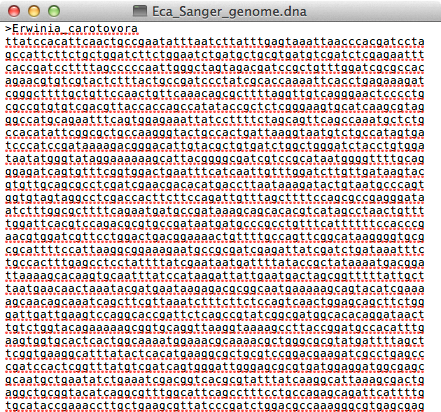
\includegraphics[height=0.5\textheight]{images/pba_sequence}
        
\includegraphics[width=0.5\textheight]{images/campy_presence_absence}
      \end{center}      
\end{frame}

% Pba
\subsection{Erwinia carotovora subsp. atroseptica}

% The sequencing project, and what we got out of it
\begin{frame}
  \frametitle{2003: \textit{E. carotovora} subsp. \textit{atroseptica}}
  \begin{itemize}
    \item \textbf{ \pounds250k collaboration} between SCRI, University of Cambridge, WT Sanger Institute
    \item Single isolate: \textit{E. carotovora} subsp. \textit{atroseptica} SCRI1043
    \item The first sequenced enterobacterial plant pathogen (32 authors!) \footnote{\tiny{Bell \textit{et al}. (2004) \textit{Proc. Natl. Acad. Sci. USA} \textbf{101}: \textbf{30}:11105-11110. \href{http://dx.doi.org/10.1073/pnas.0402424101}{doi:10.1073/pnas.0402424101}}}\\ 
      \begin{center}
        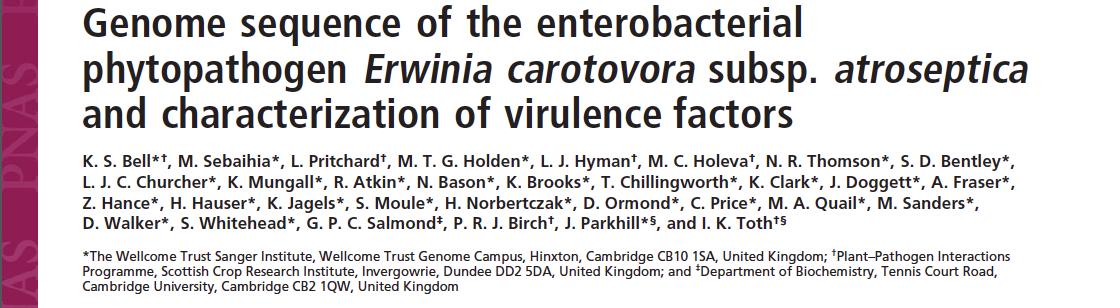
\includegraphics[width=0.6\textwidth]{images/pba_pnas}
      \end{center}    
    \item All repeats and gaps bridged and sequenced directly
    \item \textbf{Result}: a single, complete, high-quality 5Mbp circular chromosome at 10.2X coverage: 106,500 reads
  \end{itemize}
\end{frame}

% The effort that went into annotation
\begin{frame}
  \frametitle{2003: \textit{E. carotovora} subsp. \textit{atroseptica}}
  A genome sequence is a starting point$\ldots$
  \begin{itemize}
    \item Manual annotation by the Sanger Pathogen Sequencing Unit
    \item Literature searches and comparisons
    \item \textbf{Six people, for six months $\approx$ three person-years}
    \item Genes: \texttt{BLAST}, \texttt{GLIMMER}, \texttt{ORPHEUS}
    \item Functional domains: \texttt{PFAM}, \texttt{SIGNALP}, \texttt{TMHMM}
    \item Metabolism: \texttt{KEGG}
    \item ncRNA: \texttt{RFAM}
  \end{itemize}
\end{frame}

% Annotation files
\begin{frame}
  \frametitle{2003: \textit{E. carotovora} subsp. \textit{atroseptica}}
  Working (\url{Eca_Sanger_annotation.gbk}) and published (\url{NC_004547.gbk}) annotation files are in the \texttt{data} directory
  \begin{center}
    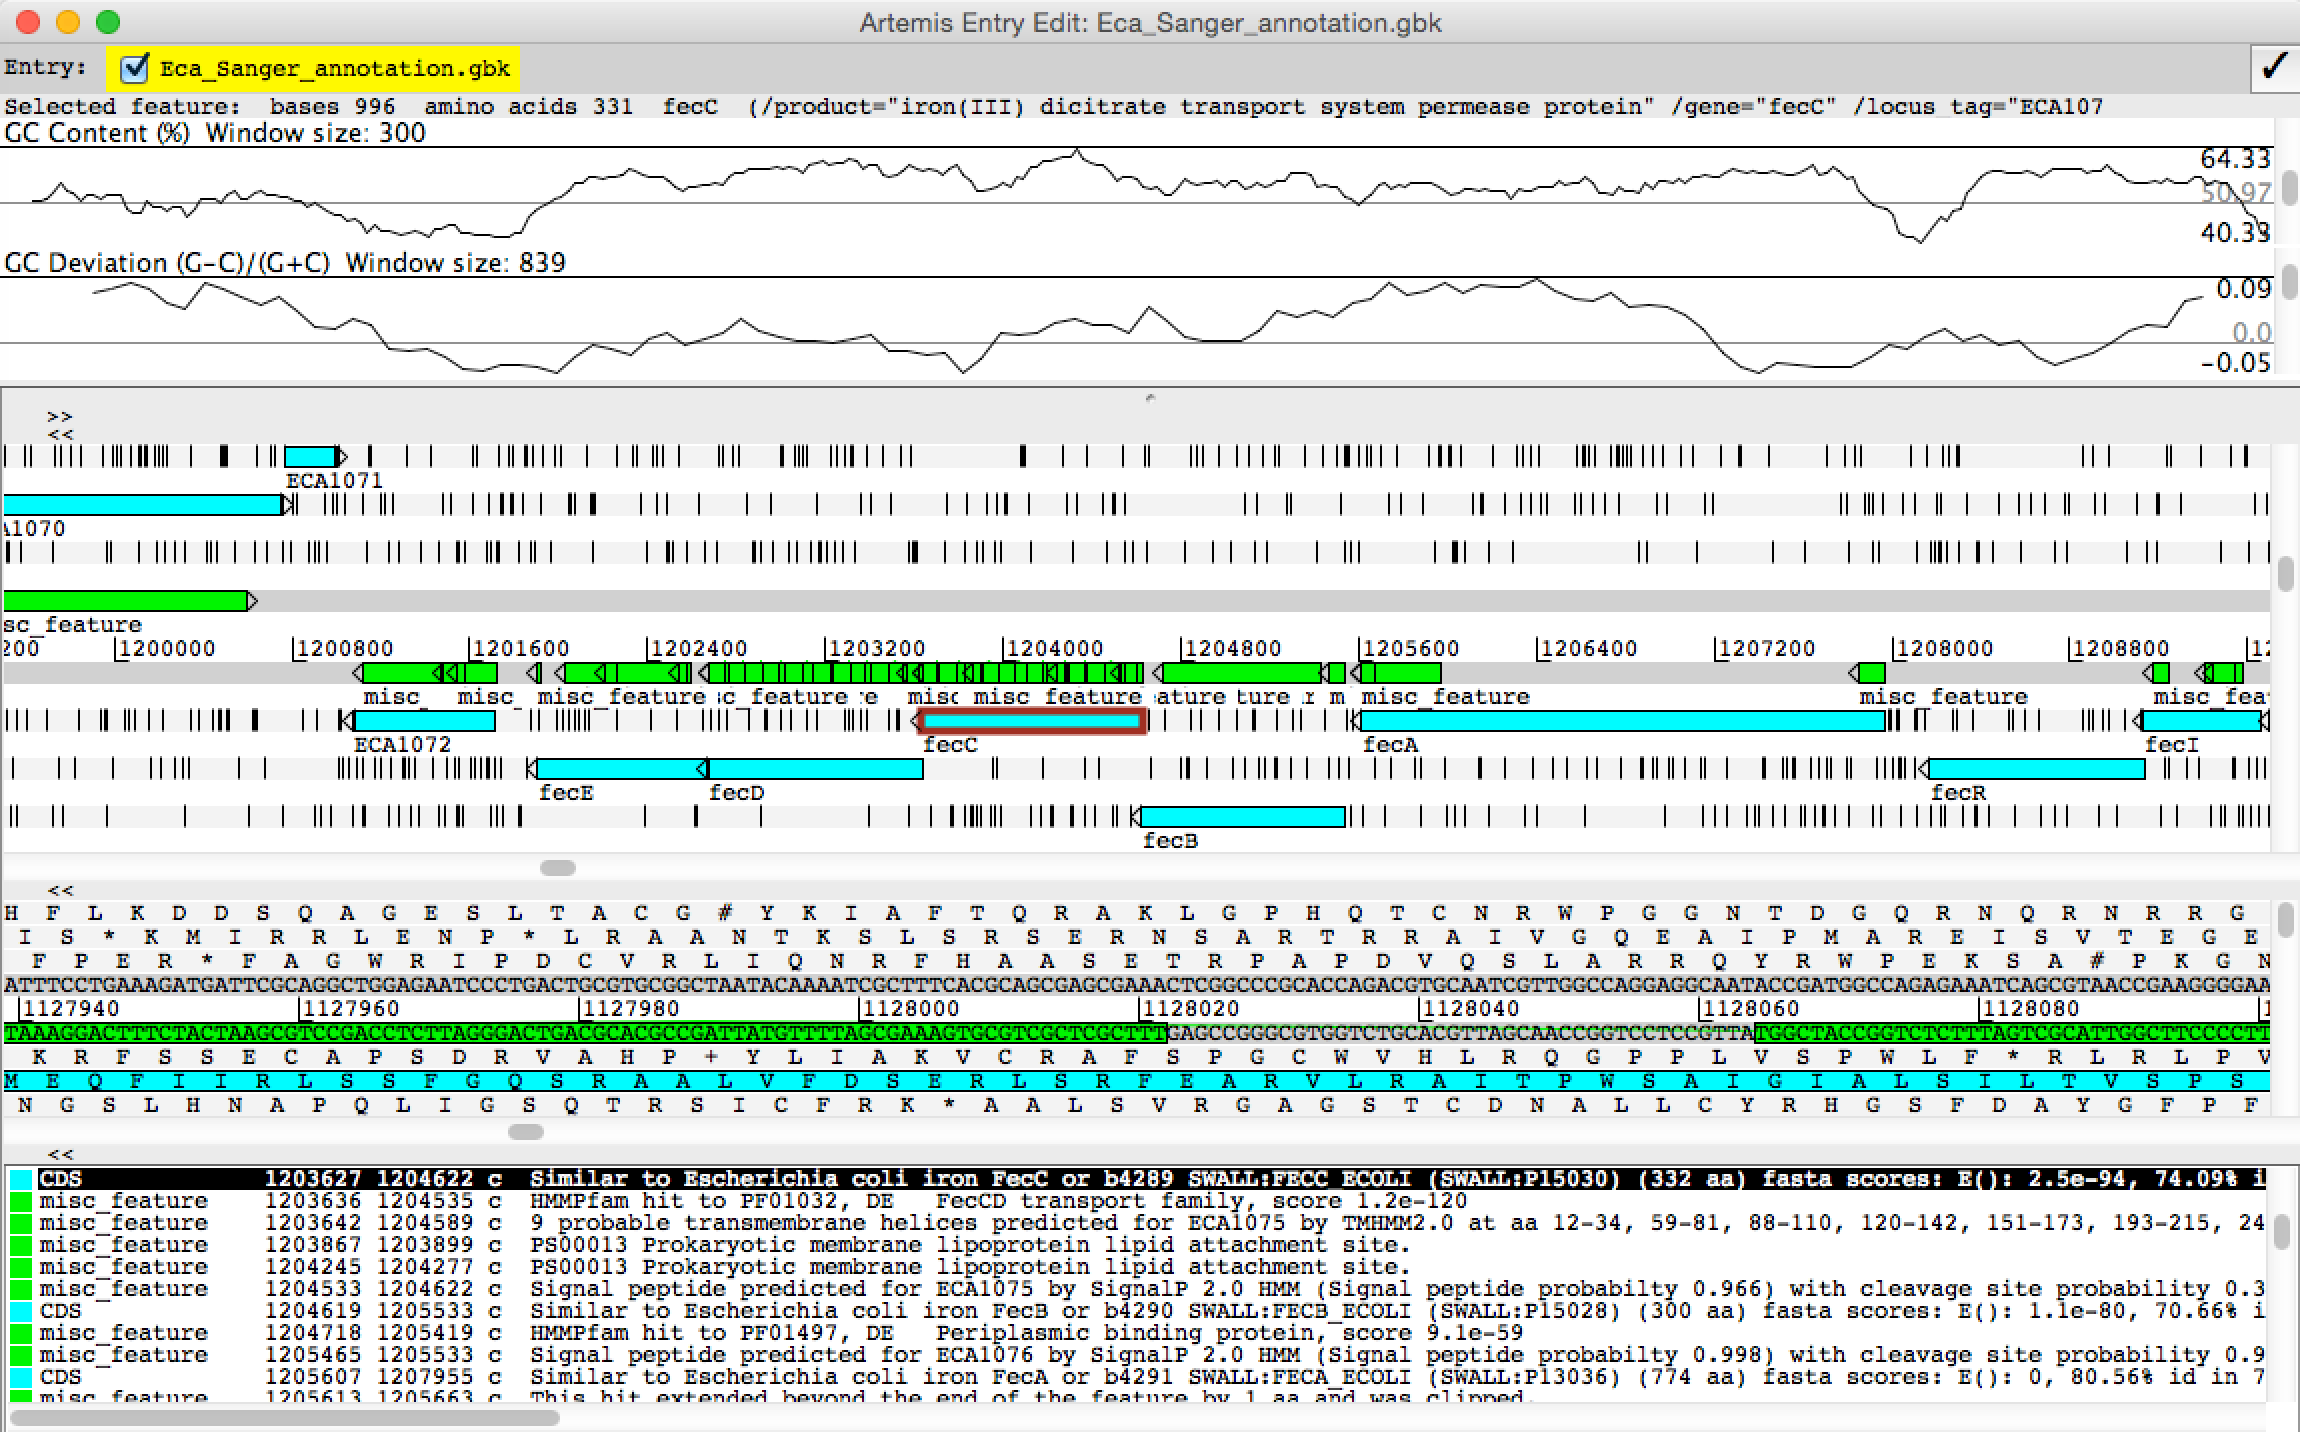
\includegraphics[width=0.9\textwidth]{images/pba_artemis}
  \end{center}    
\end{frame}

% The comparative genomics
\begin{frame}
  \frametitle{2003: \textit{E. carotovora} subsp. \textit{atroseptica}}
  Compared against all 142 available bacterial genomes\footnote{\tiny{\url{data/Pba} directory in the accompanying GitHub repository}}
  \begin{center}
    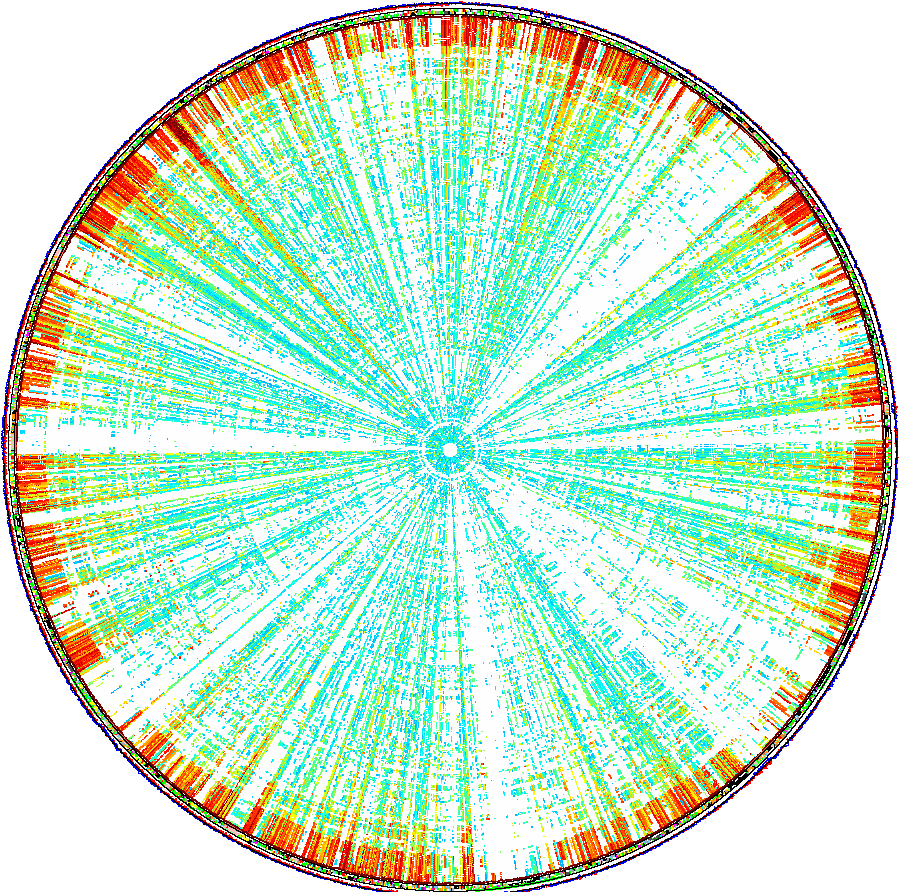
\includegraphics[width=0.6\textwidth]{images/pba_400_circular}
  \end{center}    
\end{frame}

% Dickeya etc
\subsection{Dickeya spp., Campylobacter spp., and Escherichia coli}

% Dickeya sequencing summary
\begin{frame}
  \frametitle{2013: \textit{Dickeya} spp.}
  Sequenced and annotated 25 new isolates of \textit{Dickeya}
  \begin{itemize}
    \item 25 \textit{Dickeya} isolates, at least six species
    \item Multiple sequencing methods: 454, Illumina (SE, PE)
    \item Minor publications (6, 8 authors)%
\footnote{\tiny{Pritchard \textit{et al}. (2013) \textit{Genome Ann.} \textbf{1} (4) \href{http://dx.doi.org/10.1128/genomeA.00087-12}{doi:10.1128/genomeA.00087-12}}}$^{,}$%
\footnote{\tiny{Pritchard \textit{et al}. (2013) \textit{Genome Ann.} \textbf{1} (6) \href{http://dx.doi.org/10.1128/genomeA.00978-13}{doi:10.1128/genomeA.00978-13}}}\\ 
      \begin{center}
        
\includegraphics[width=0.5\textwidth]{images/dickeya_ga1}
        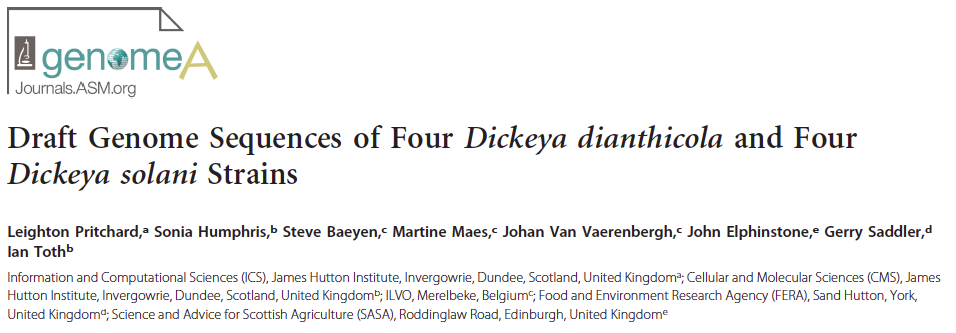
\includegraphics[width=0.5\textwidth]{images/dickeya_ga2}
      \end{center}    
    \item \textbf{Results}: 12-237  fragments containing 4.2-5.1Mbp, at 6-84X coverage, 170k-4m reads
    \item \textbf{Automated annotation: RAST} with manual corrections
  \end{itemize}  
\end{frame}

% Dickeya sequencing summary
\begin{frame}
  \frametitle{2013: \textit{Dickeya} spp.}
  Within-genus comparisons: large-scale synteny and rearrangement
  \begin{center}
    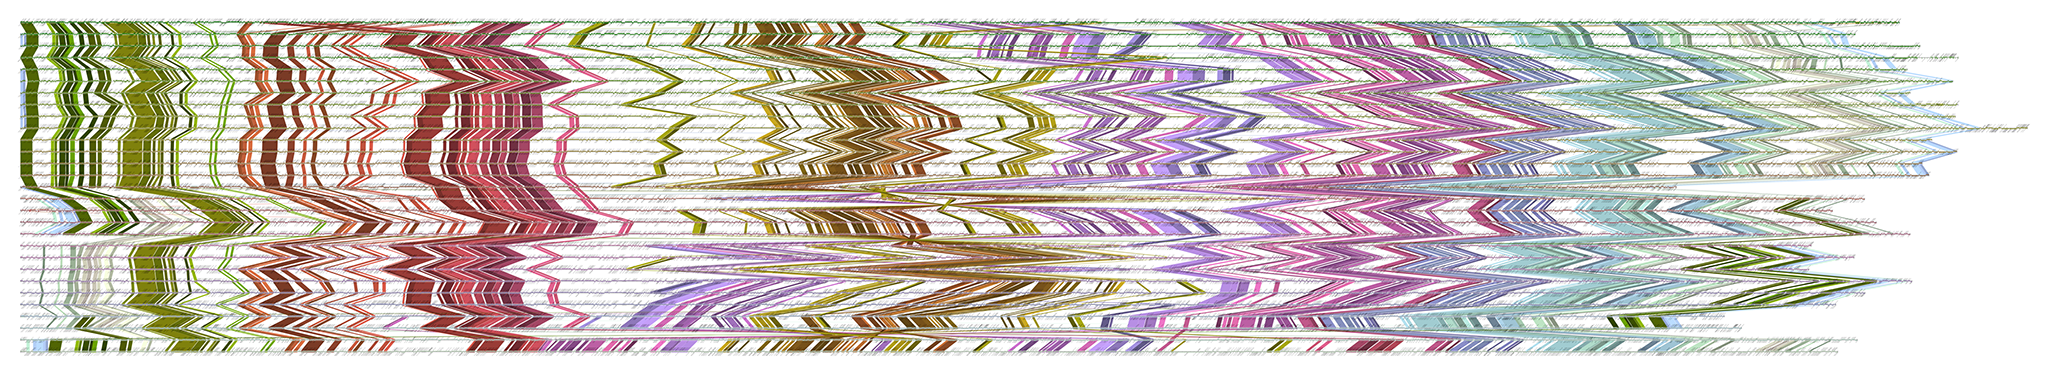
\includegraphics[width=1\textwidth]{images/dickeya_core_collinear_small}
  \end{center}    
  Within-species comparisons: e.g. indels, HGT
  \begin{center}
    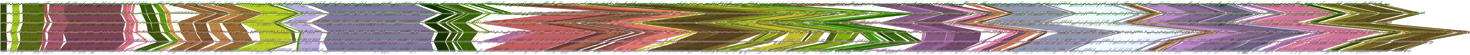
\includegraphics[width=1\textwidth]{images/collinear_zeae}
  \end{center}      
\end{frame}

% Dickeya sequencing summary
\begin{frame}
  \frametitle{2013: \textit{Dickeya} spp.}
  Within-genus comparisons: whole genome-based species delineation\footnote{\tiny{\href{http://dx.doi.org/10.1099/ijs.0.052944-0}{van der Wolf \textit{et al}. (2014) \textit{Int. J. Syst. Evol. Micr.} \textbf{64}:768-774 doi:10.1099/ijs.0.052944-0}}}
  \begin{center}
    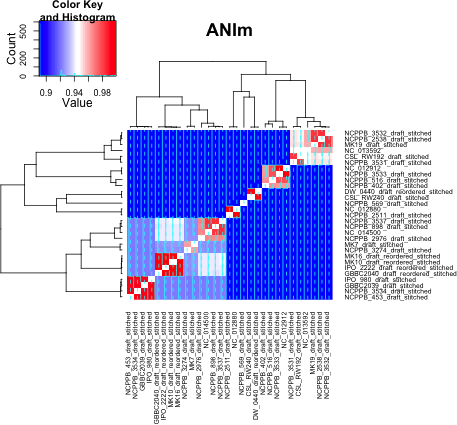
\includegraphics[width=0.6\textwidth]{images/dickeya_ani}
  \end{center}      
\end{frame}

% E.coli sequencing summary
\begin{frame}
  \frametitle{2014: \textit{E. coli}}
  Sequenced and annotated $\approx$ 190 isolates of \textit{E. coli} \\
  All bacteria environmental, sampled from lysimeters
  \begin{itemize}
    \item Illumina paired-end sequencing. \textbf{Total cost of sequencing 190 bacteria: $\approx$\pounds11k}
    \item \textbf{Automated annotation: PROKKA}
  \end{itemize}  
\end{frame}

% E.coli sequencing variation
\begin{frame}
  \frametitle{2014: \textit{E. coli}}
  Sequencing output variable - even though same preps, ``same'' bacteria, similar sources.
  \begin{itemize}
    \item \textbf{Results}: 5-3000 contigs (median $\approx$ 125); 9kbp-7.1Mbp (median $\approx$ 5Mbp); 170k-4m reads
  \end{itemize}  
  \begin{center}
    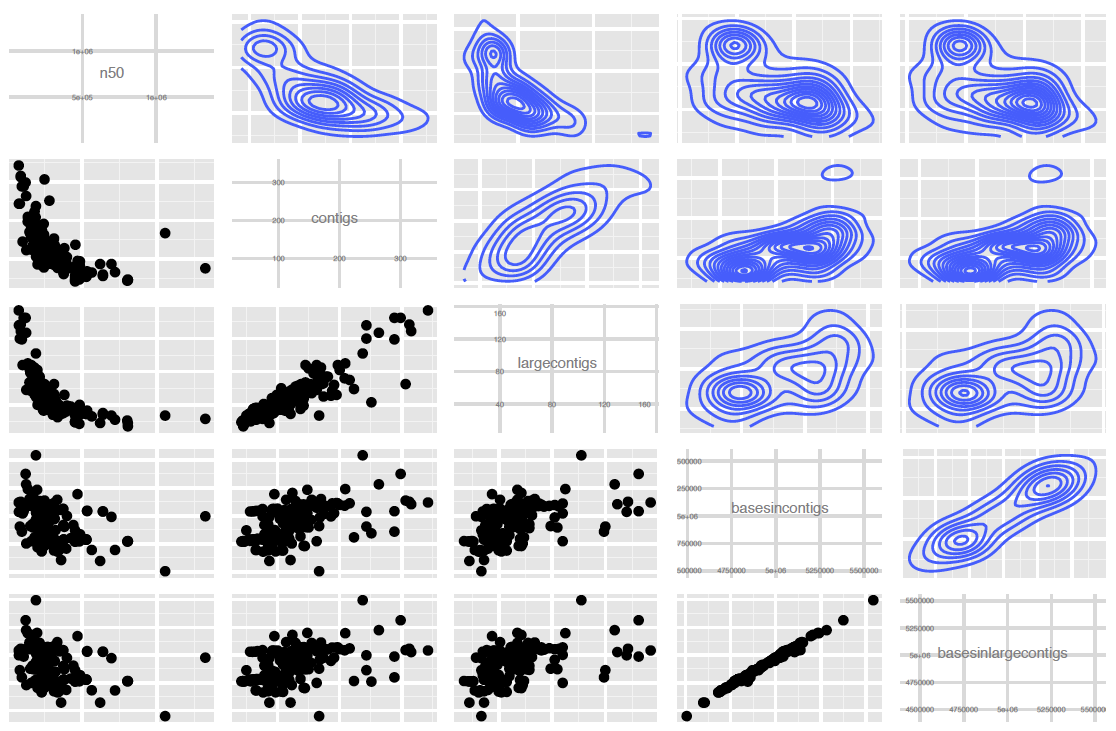
\includegraphics[width=0.7\textwidth]{images/ecoli_sequencing_variation}
  \end{center}      
\end{frame}

% E.coli within-species variation
\begin{frame}
  \frametitle{2014: \textit{E. coli}}
  Genome sequencing enables within-species classification
  \begin{center}
    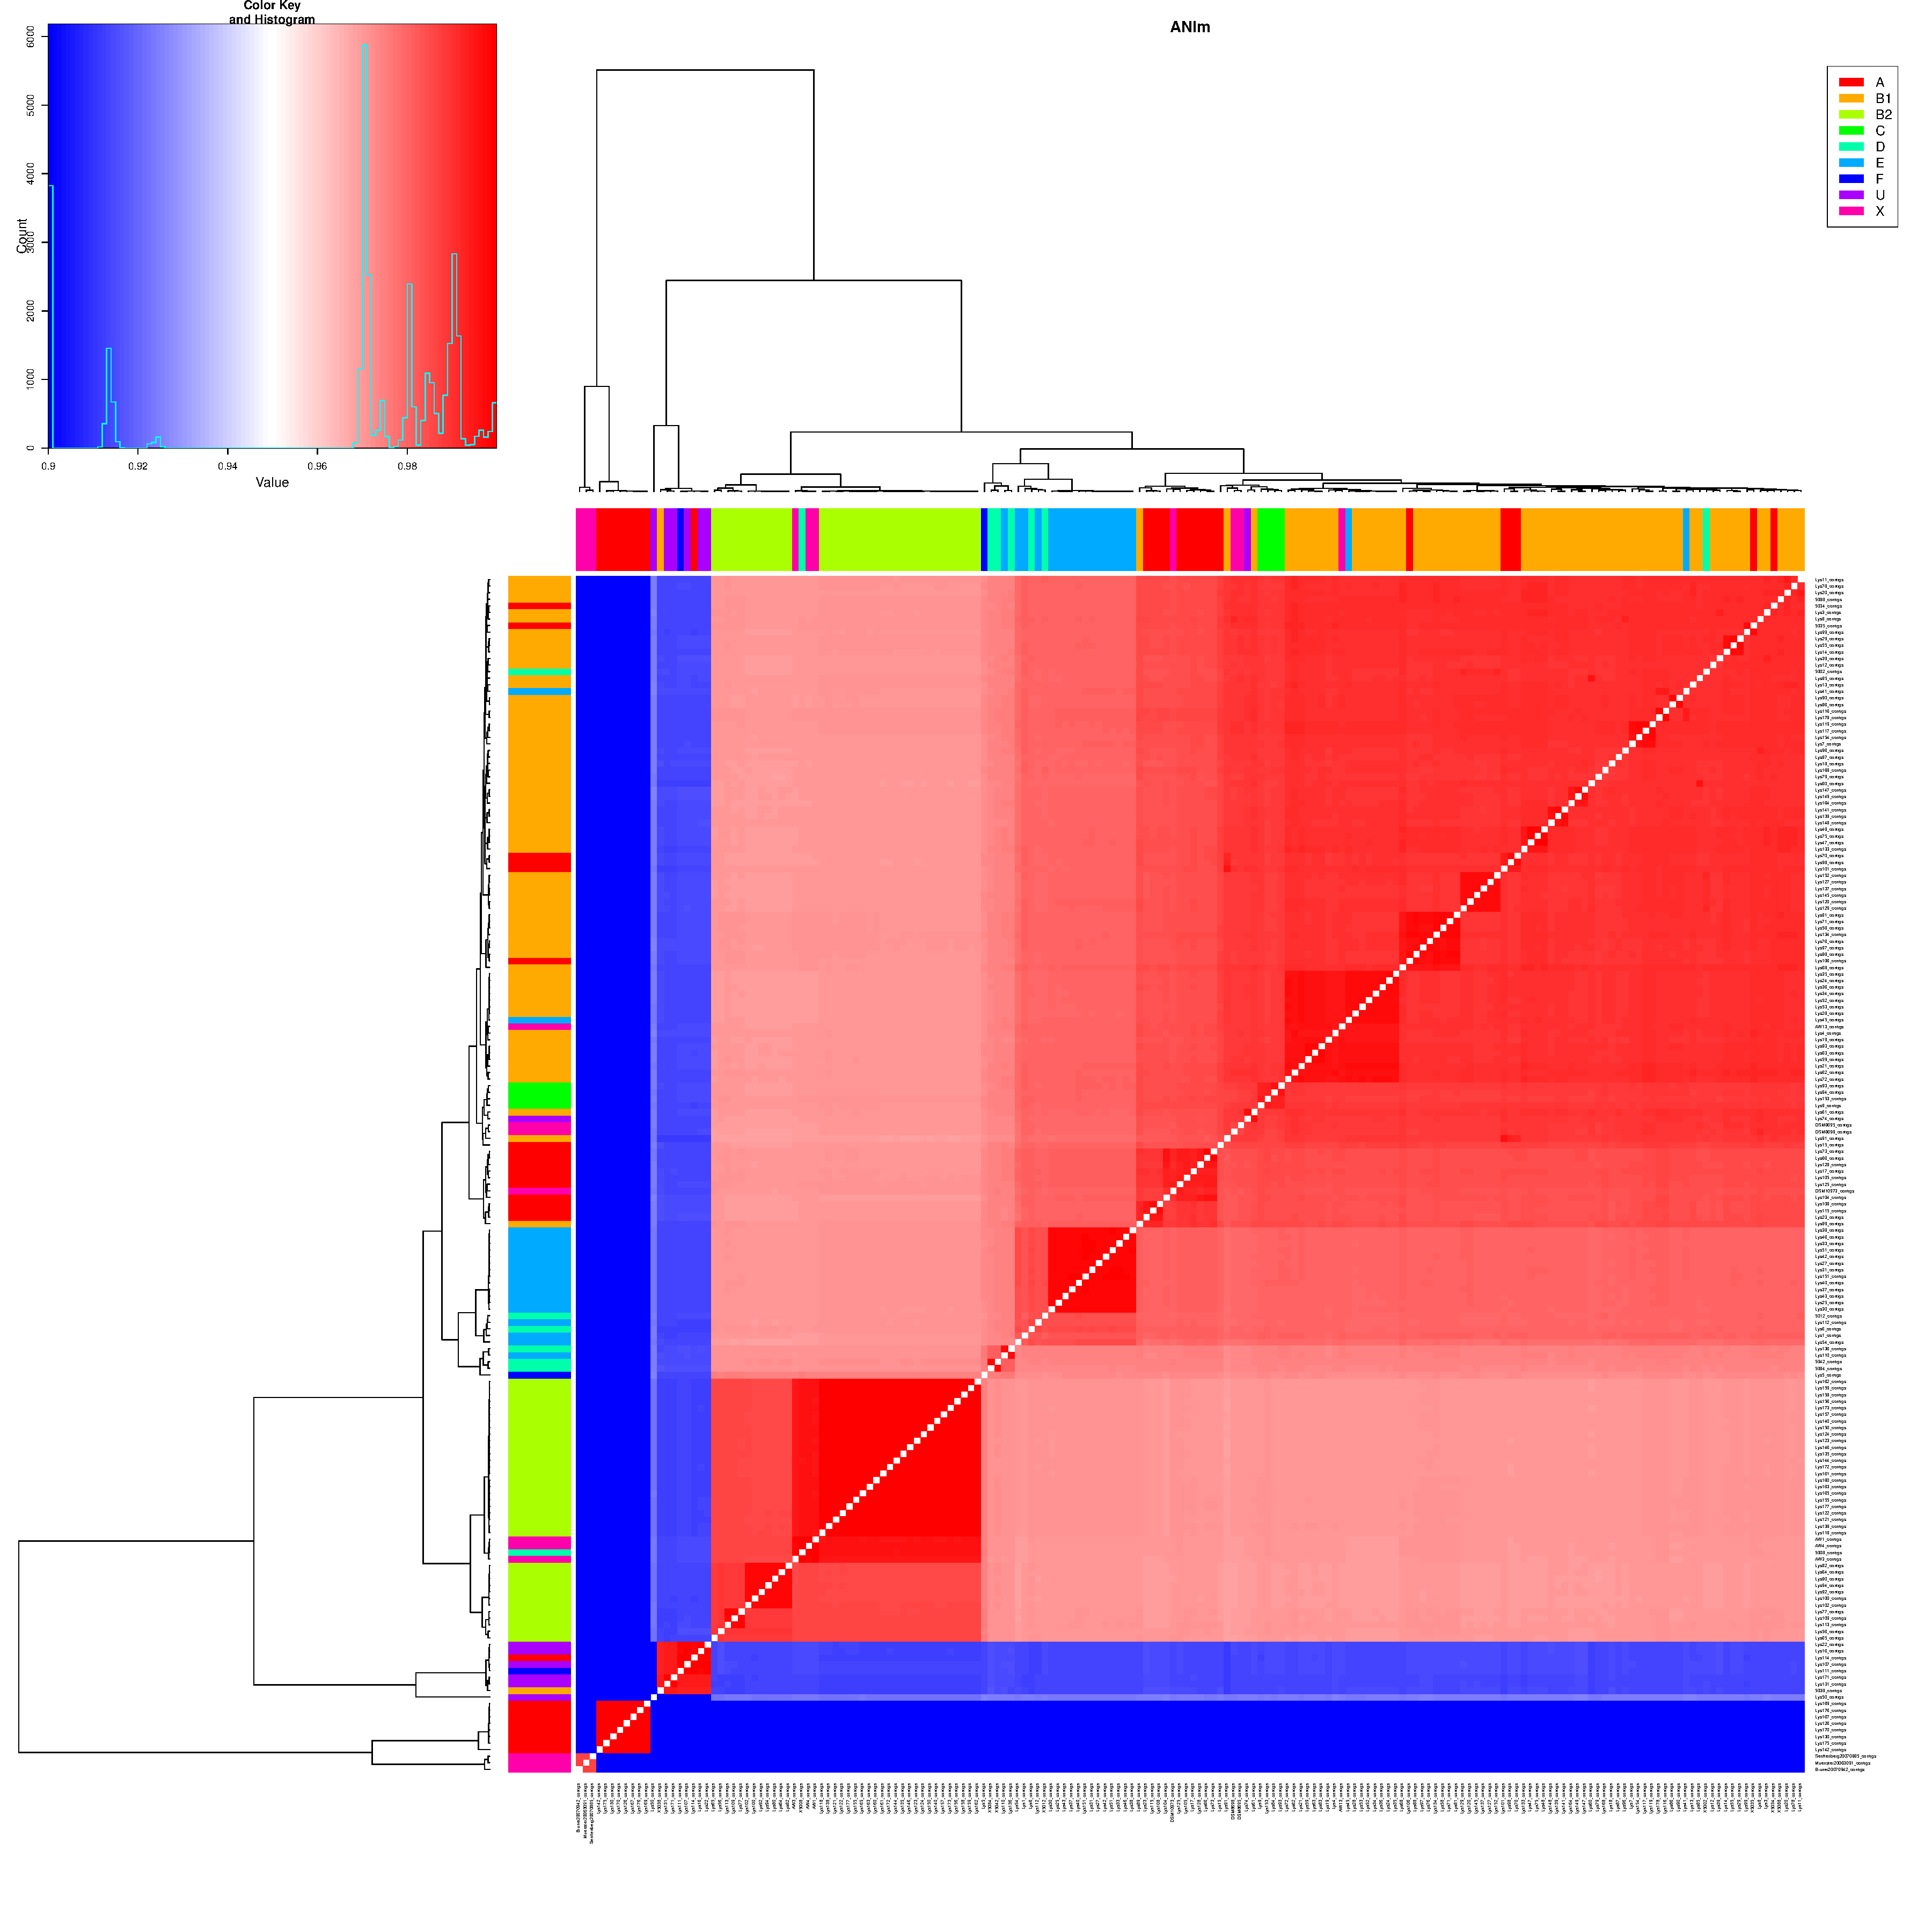
\includegraphics[width=0.65\textwidth]{images/ANIm_Ecoli}
  \end{center}      
\end{frame}

% Campy sequencing summary
\begin{frame}
  \frametitle{2014: \textit{Campylobacter} spp.}
  Sequenced $\approx$ 1034 isolates of \textit{Campylobacter} \\
  Clinical, animal, food-associated isolates
  \begin{itemize}
    \item Illumina paired-end sequencing. \textbf{Total cost of sequencing $>$1000 bacteria: $\approx$\pounds60k}
    \item \textbf{Automated annotation: PRODIGAL}    
  \end{itemize}      
  \begin{center}
    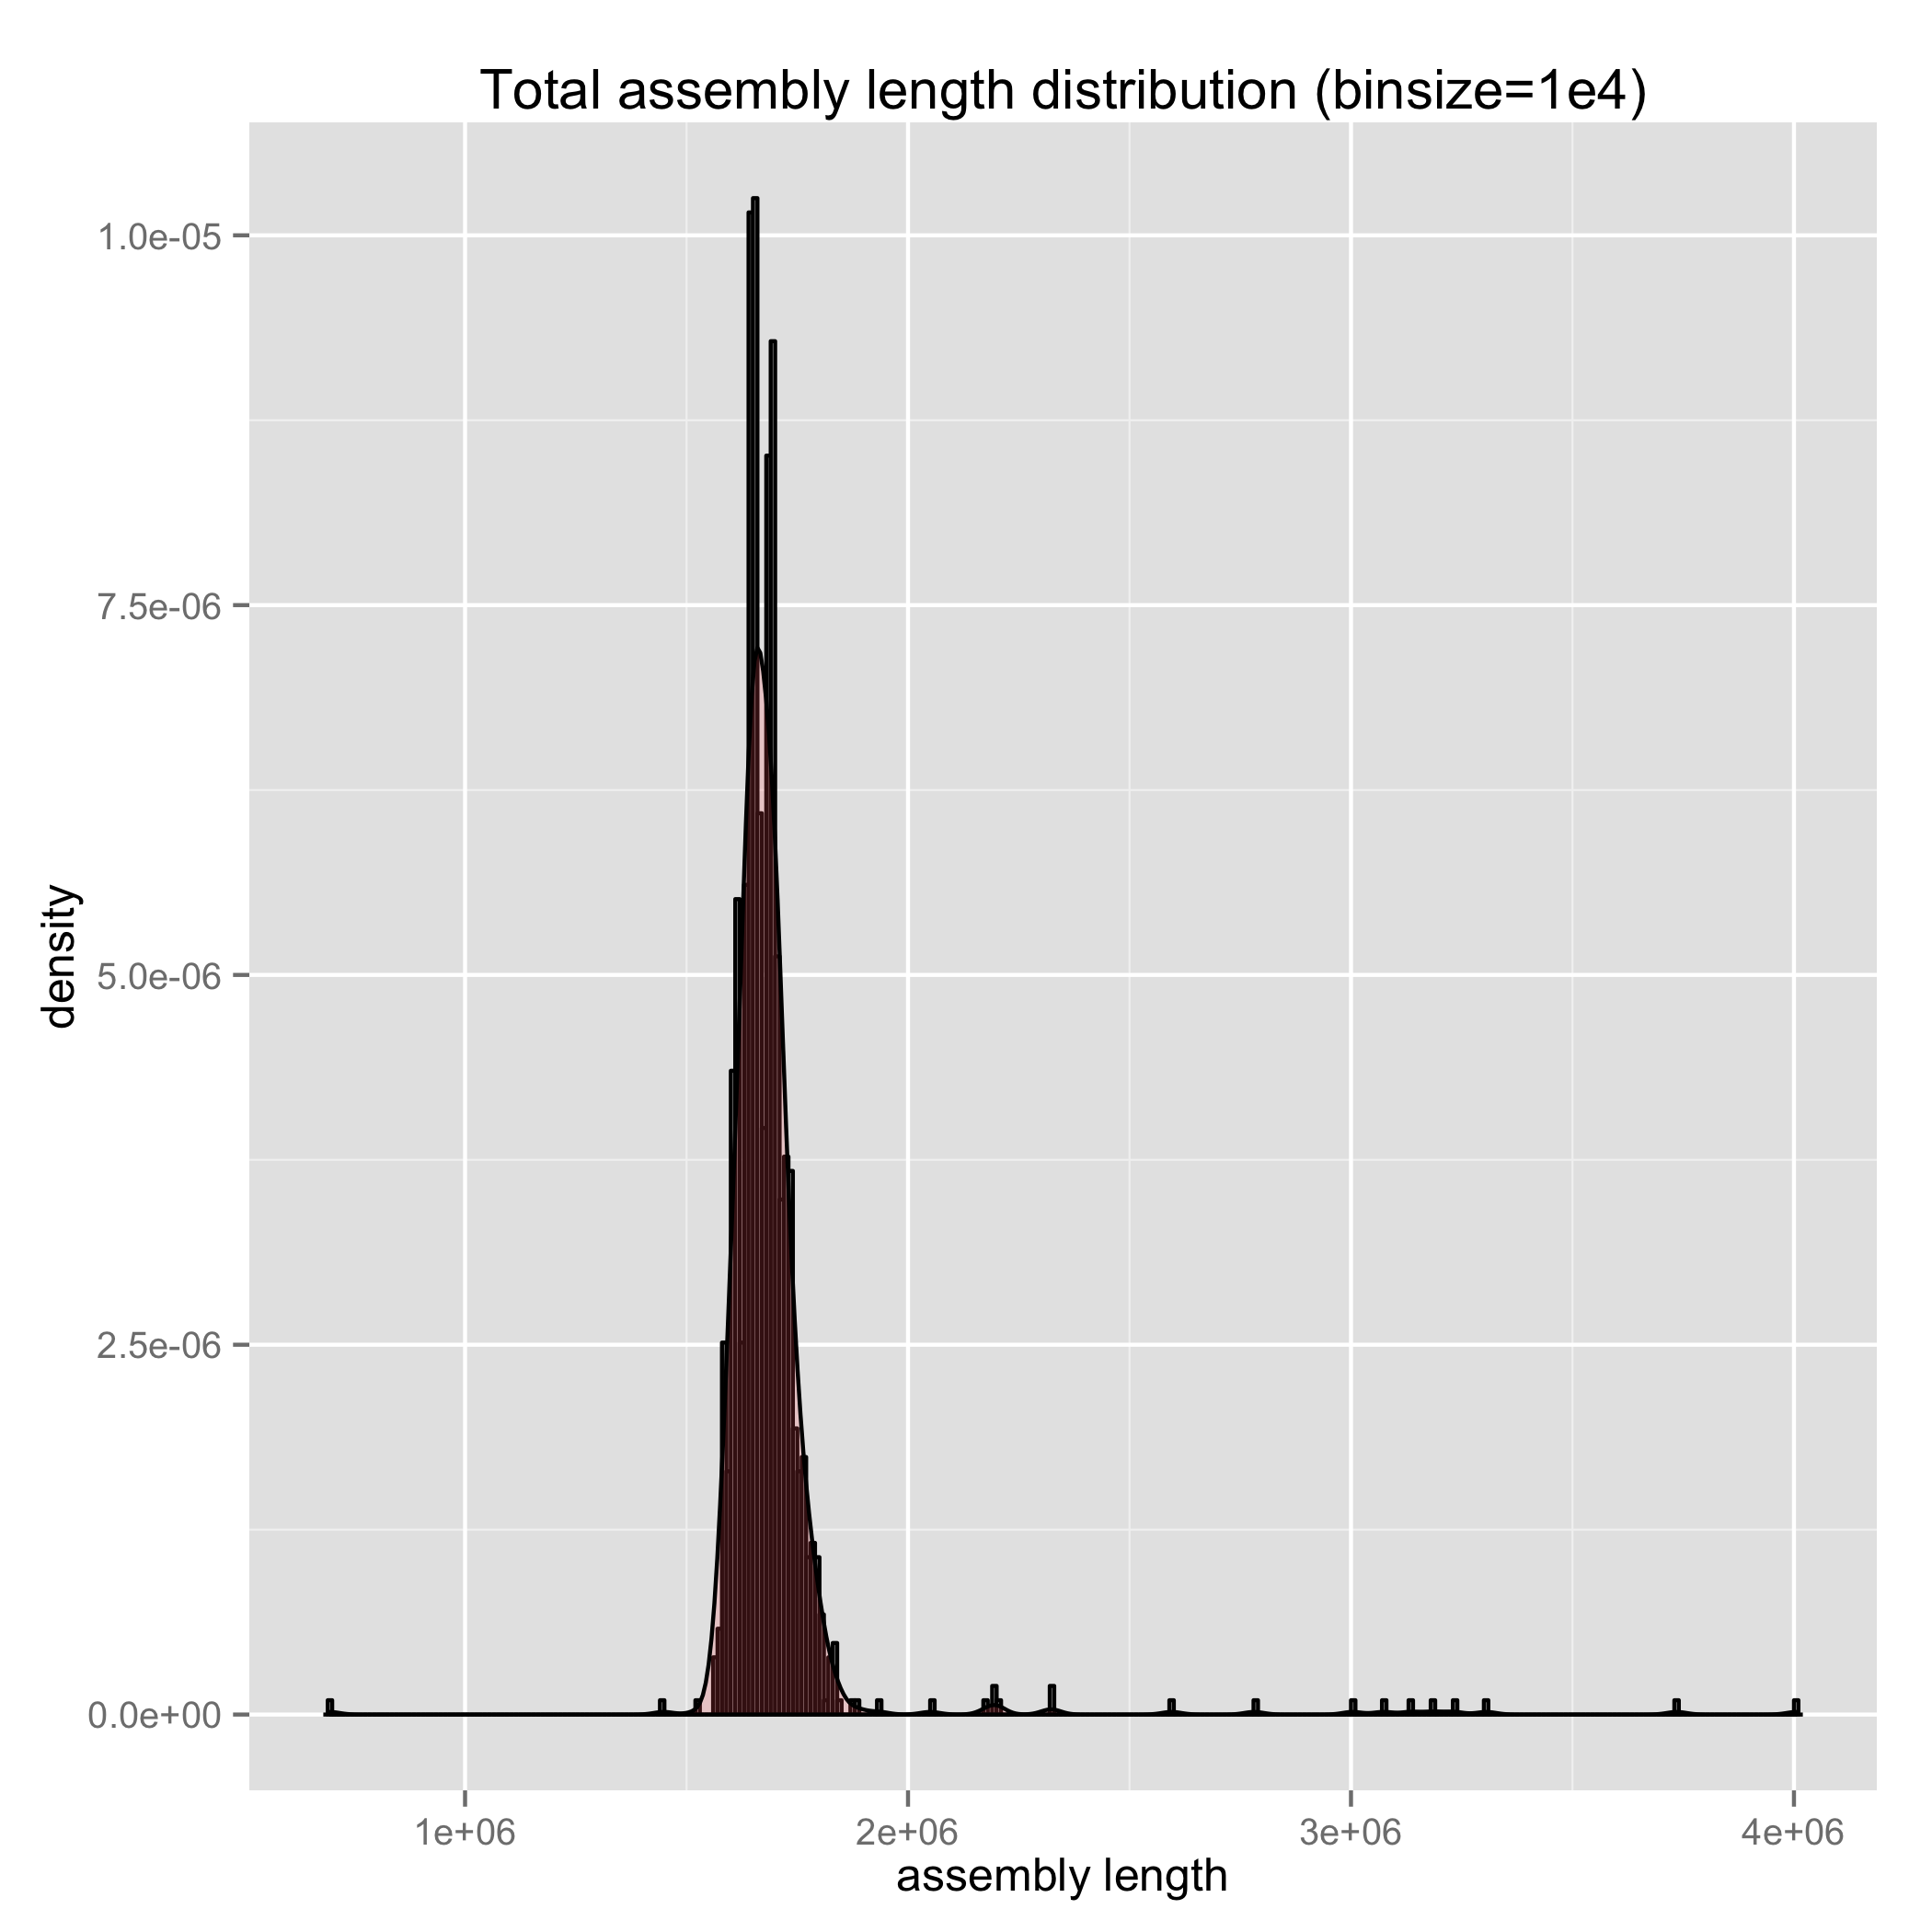
\includegraphics[width=0.4\textwidth]{images/Asm_long_contigs_length_histogram}
  \end{center}        
\end{frame}

% Campy genecalling summary
\begin{frame}
  \frametitle{2014: \textit{Campylobacter} spp.}
  \begin{itemize}
    \item Identified 15554 gene families from genecalls.
    \item To calculate, took 23 days on institute cluster (4e12 pairwise protein comparisons!).  
  \end{itemize}      
  \begin{center}
    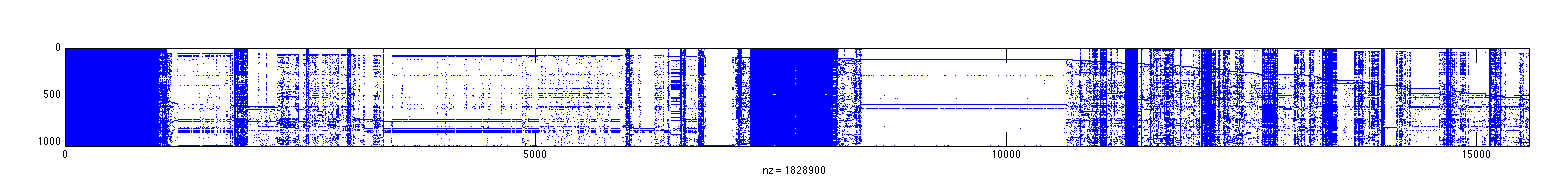
\includegraphics[width=1\textwidth]{images/Pres_abs_mat} \\
    
\includegraphics[width=0.4\textwidth]{images/campy_presence_absence}    
  \end{center}        
\end{frame}

% SUBSECTION: What's changed?
% What are the major changes that 
\subsection{So what's changed?}

% High-throughput sequencing totally changed everything
\begin{frame}
  \frametitle{So what's changed?}
  \begin{itemize}
    \item \textbf{Cost}: \pounds250k per genome, to \pounds60 per genome. \\
             \textbf{Now cheaper to sequence a genome than to analyse it!}
    \item \textbf{Location}: sequencing centre, to benchtop
    \item \textbf{Data}: volume has increased massively - what you get back from machines, and what's out there to work with\\
             \textbf{More data is better, but also more challenging.}
    \item \textbf{Speed}: typical sequencing run time can be less than a day
    \item \textbf{Software}: more software to do more things (but not always better$\ldots$)
    \item New kinds of \textbf{experiment}: genomes, exomes, variant calling, methylated sequences, $\ldots$
    \item New kinds of \textbf{application}: diagnostics, epidemic tracking, metagenomics, $\ldots$
  \end{itemize}       
\end{frame}

% More power for comparative genomics
\begin{frame}
  \frametitle{So what's changed?}
  Having a single genome is useful, but having thousands really helps \textbf{\textit{comparative genomics}}: \\
  combining genomic data, evolutionary and comparative biology
  \begin{itemize}
    \item Transfer functional understanding of model systems (e.g. \textit{E. coli}) to non-model organisms
    \item Genomic differences may underpin phenotypic (host range, virulence, physiological) differences
    \item Genome comparisons aid identification of functional elements on the genome
    \item Studying genomics changes reveals evolutionary processes and constraints
  \end{itemize}       
\end{frame}



\section{High Throughput Sequencing}
%% high_throughput_sequencing.tex
%% Author: Leighton Pritchard
%% Copyright: James Hutton Institute
%% These slides briefly introduce the four main sequencing technologies
%% and comment on their relative performance and price.
%% Next they mention Oxford Nanopore as the next promising technology,
%% and the potential impact it could have on sequencing.
%% Finally, the impact that this technology has had on databases and 
%% analyses etc. are described.

% SUBSECTION: Four dominant technologies
% A summary of the characteristics of the four dominant sequencing 
% technologies, and how they can be benchmarked
\subsection{Four dominant technologies}

% The four main current sequencing technologies
\begin{frame}
  \frametitle{Not all ``sequencing'' is the same}
  Sequencing technology affects your sequence data
  \begin{itemize}
    \item Roche/454 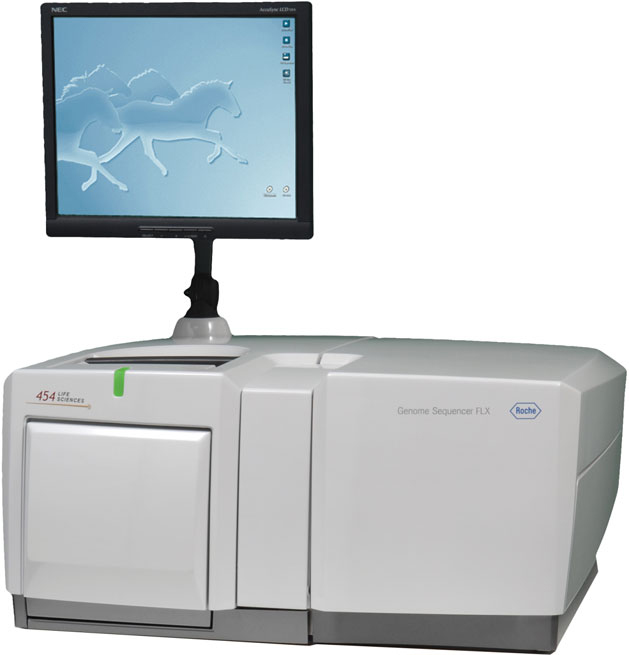
\includegraphics[height=0.15\textheight]{images/454_sequencer}
    \item Illumina 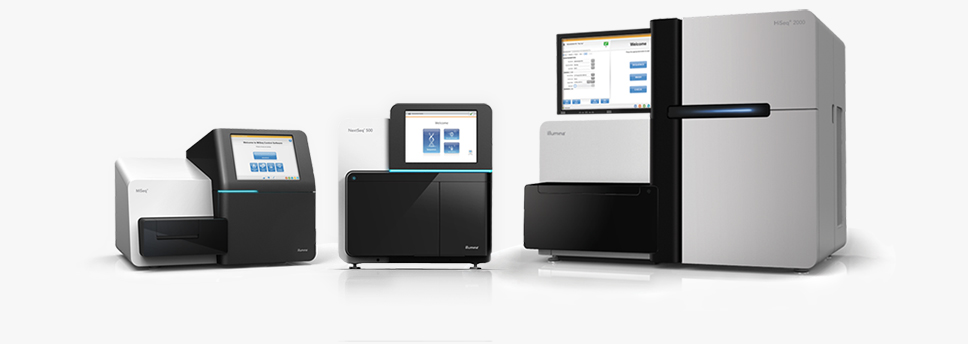
\includegraphics[height=0.15\textheight]{images/miseq_nextseq_hiseq}
    \item Ion Torrent 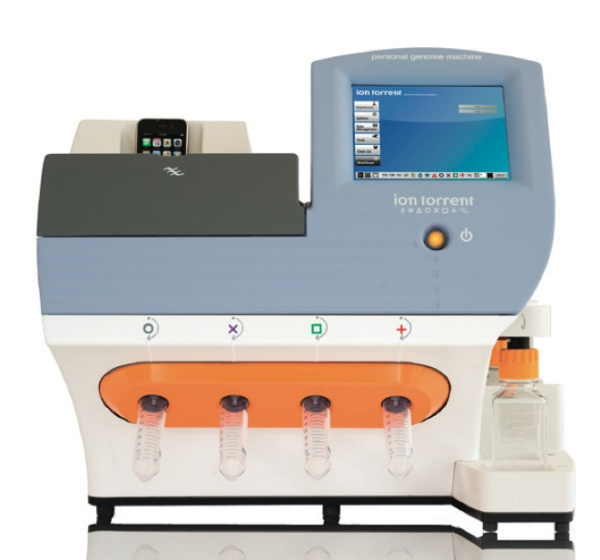
\includegraphics[height=0.15\textheight]{images/ion_torrent_personal_genome_maker}
    \item Pacific Bioscience (PacBio) 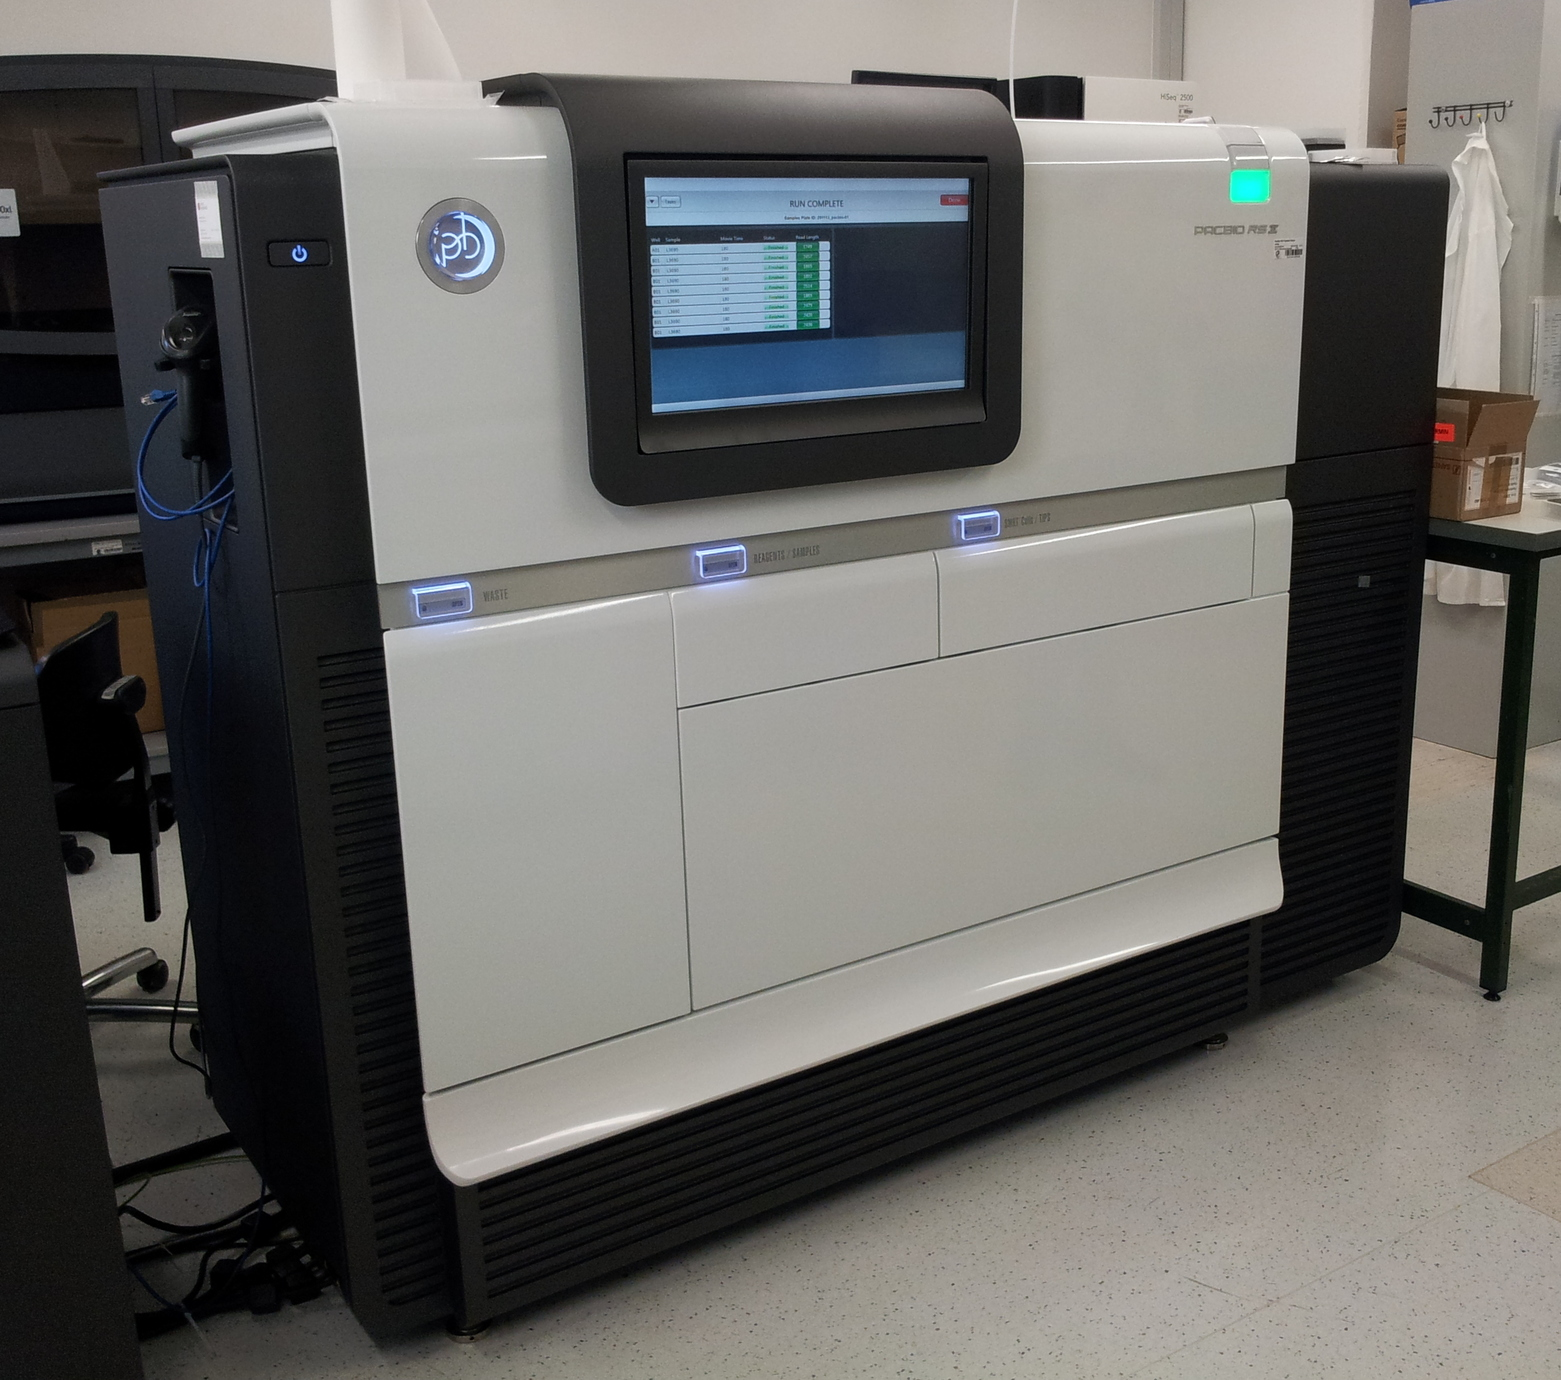
\includegraphics[height=0.15\textheight]{images/PacBio_RSII}
  \end{itemize}
\end{frame}

% Basic principle
\begin{frame}
  \frametitle{The basic principle}
  DNA source is fragmented, and the fragments are sequenced. \\
  \begin{center}
    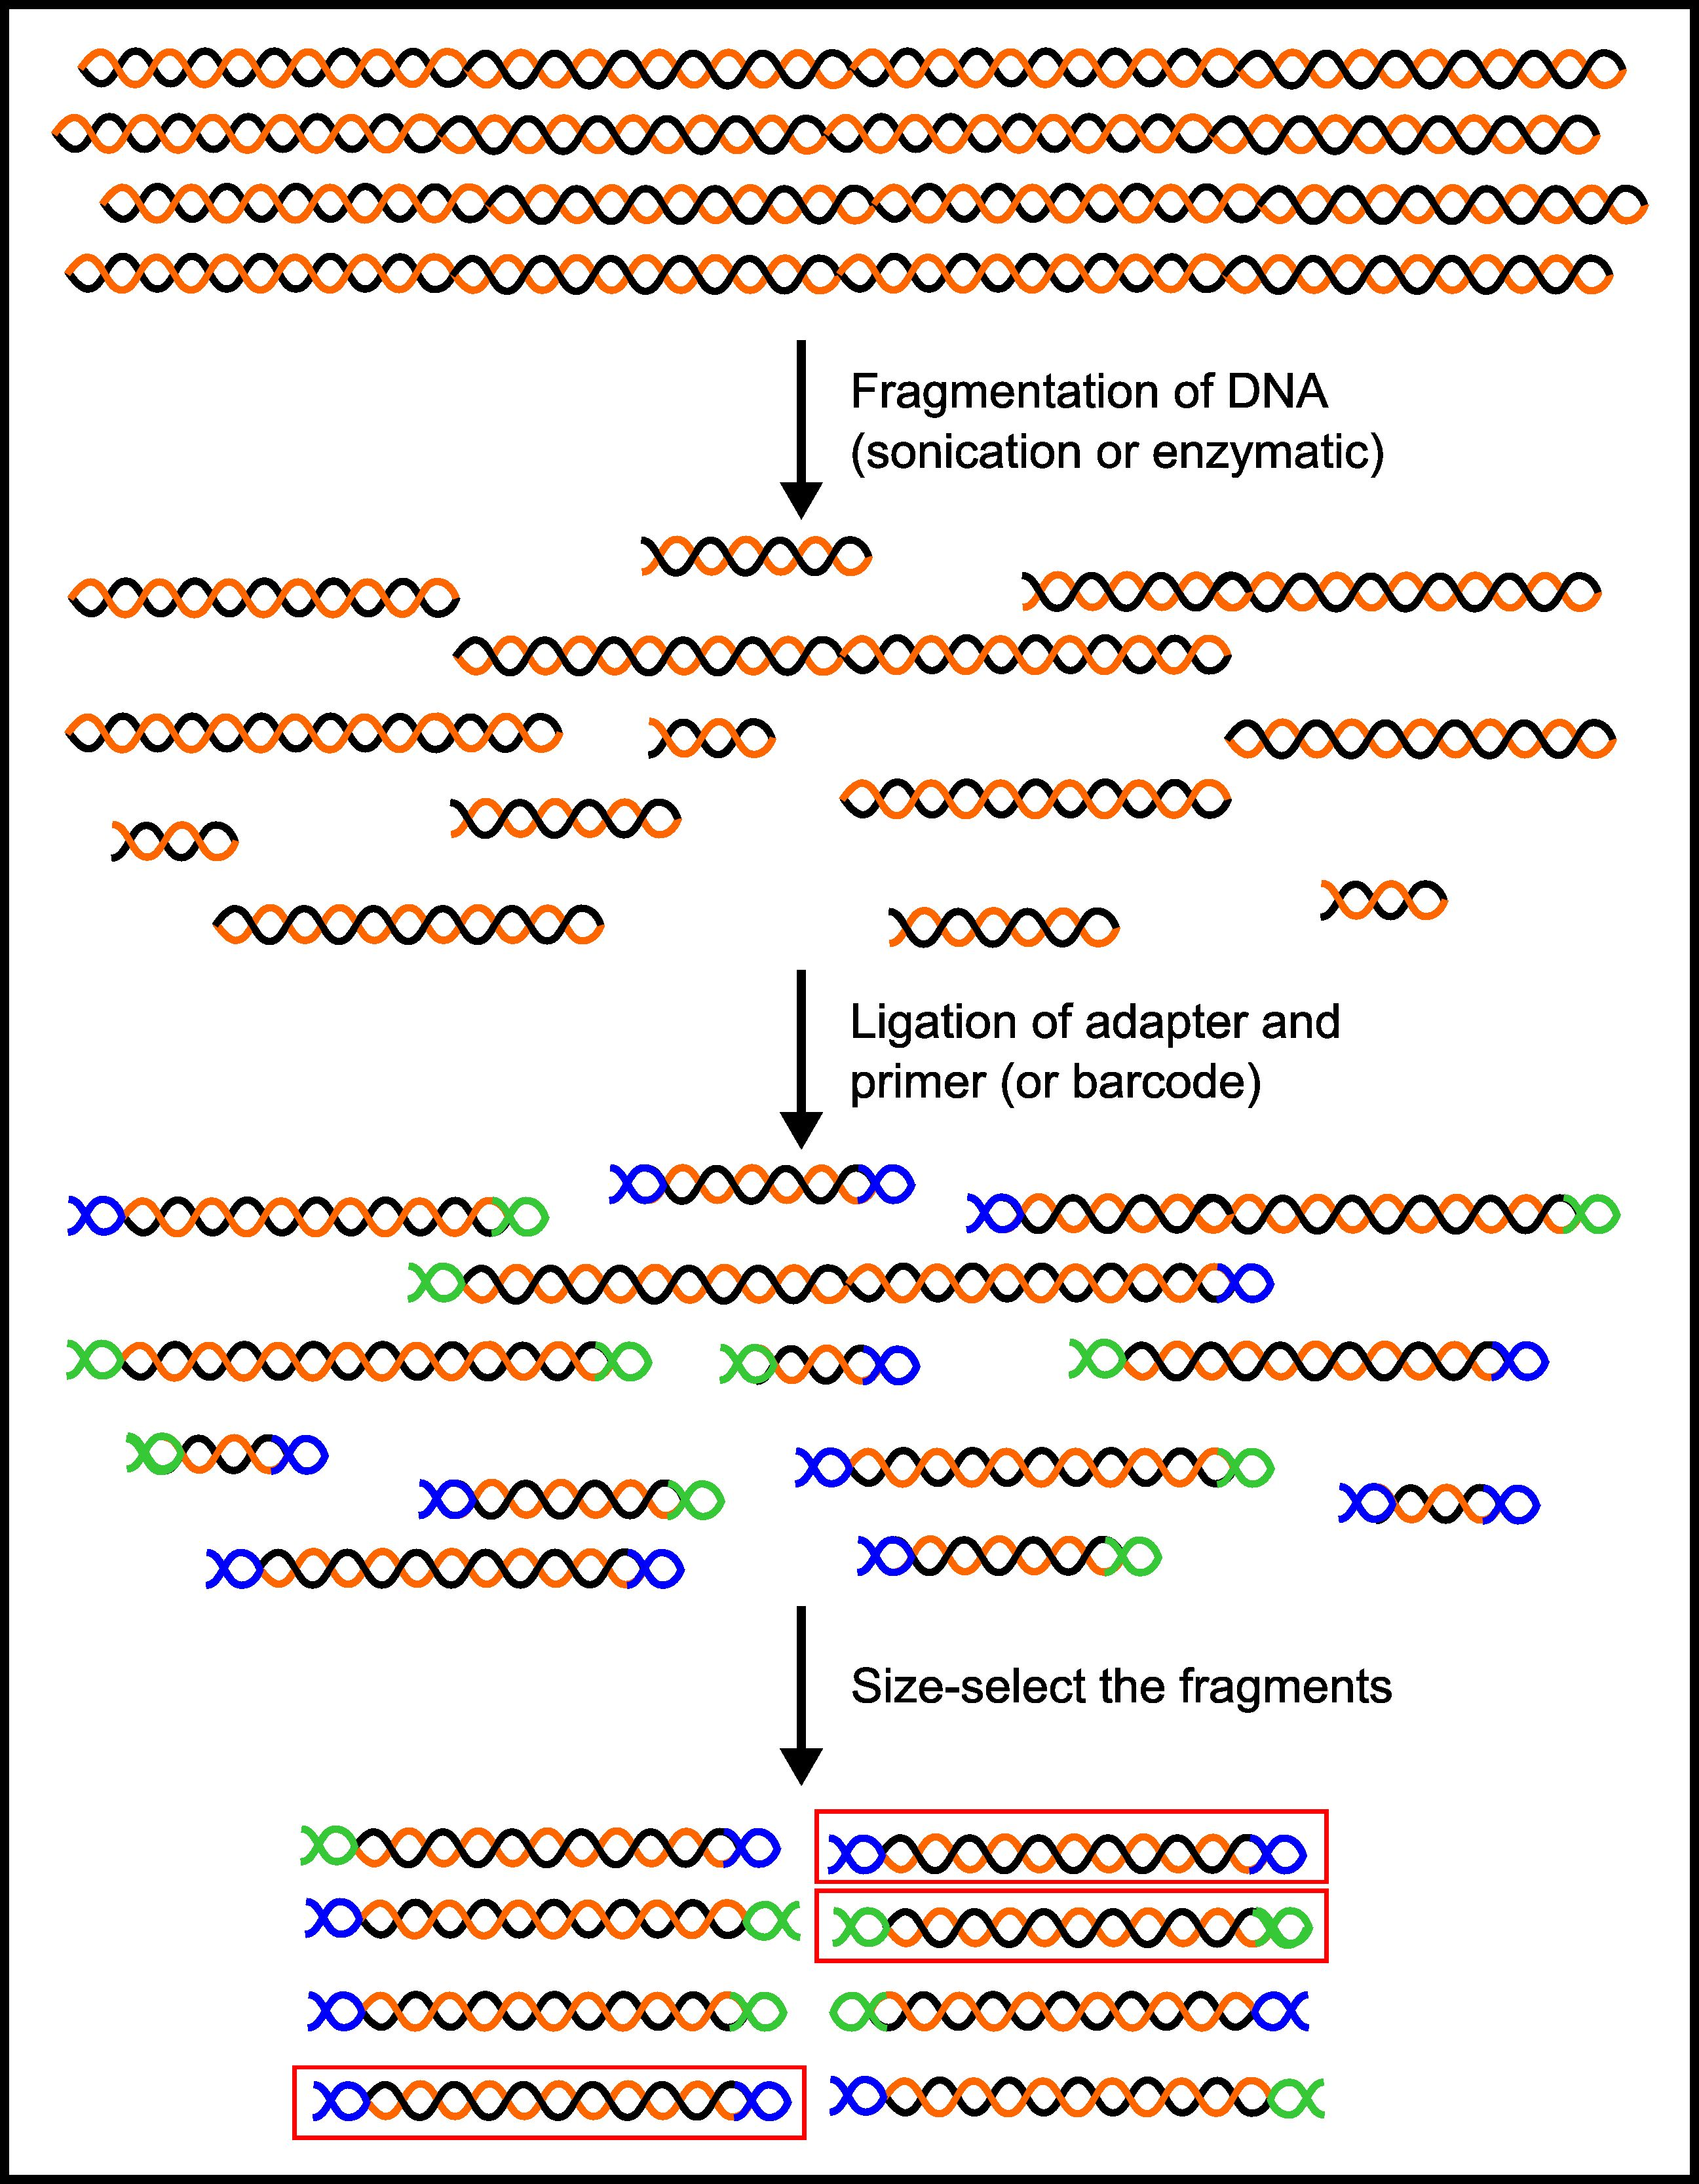
\includegraphics[height=0.7\textheight]{images/library_preparation}
  \end{center}      
\end{frame}

% Paired- and single-end reads
\begin{frame}
  \frametitle{PE vs SE}
  Reads may be single-end, or paired-end.
  \begin{center}
    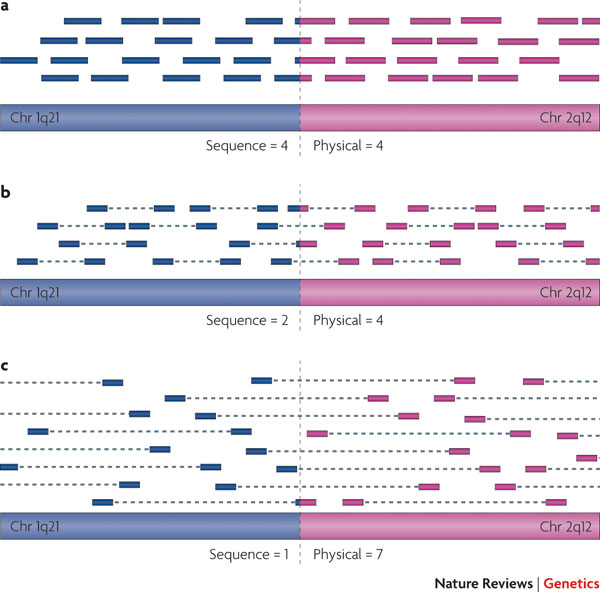
\includegraphics[height=0.6\textheight]{images/pe_vs_se}
  \end{center}      
  Putting the jigsaw back together is sequence assembly.
\end{frame}

% Broad differences in chemistry and output
\begin{frame}
  \frametitle{Four different chemistries\footnote{\tiny{Loman \textit{et al}. (2012) \textit{Nat. Rev. Micro.} \textbf{31}:294-296 \href{http://dx.doi.org/10.1038/nbt.2522}{doi:10.1038/nbt.2522}}}}
  Results differ by technology, and may require different bioinformatic treatment$\ldots$
  \begin{itemize}
    \item \textbf{Roche/454}: Pyrosequencing (long reads, but expensive, and high homopolymer errors) (700-800bp, 0.7Gbp, 23h)
    \item \textbf{Illumina}: Reversible terminator (cost-effective, massive throughput, but short read lengths) (2x150bp, 1.5Gbp, 27h)
    \item \textbf{Ion Torrent}: Proton detection (short run times, good throughput, high homopolymers errors) (200bp, 1Gbp, 3h)
    \item \textbf{PacBio}: Real-time sequencing (very long reads, high error rate, expensive) (3-15kbp, 3Gbp/day, 20min)
  \end{itemize}
  $\ldots$ different error profiles, varying capability to assemble/determine variation
\end{frame}

% Sequencer relative costs
\begin{frame}
  \frametitle{Costs of sequencing\footnote{\tiny{Miyamoto \textit{et al}. (2014) \textit{BMC Genomics} \textbf{15}:699 \href{http://dx.doi.org/10.1186/1471-2164-15-699}{doi:10.1186/1471-2164-15-699}}}}
    \begin{center}
      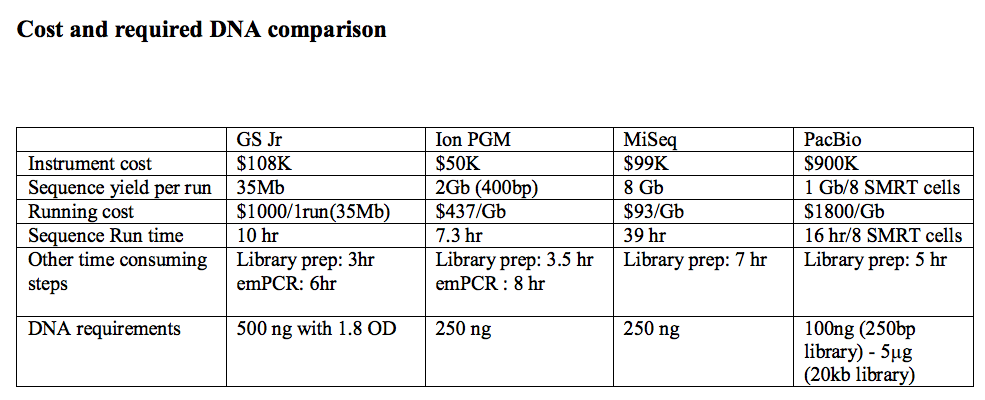
\includegraphics[width=1\textwidth]{images/miyamoto_costs}
    \end{center}      
\end{frame}

% SUBSECTION: Benchmarking
% Summary of benchmarking for sequencing methods: which is best?
\subsection{Benchmarking}

% Benchmarking is very useful
\begin{frame}
  \frametitle{Benchmarked performance}
  Apply several sequencing technologies to the same sample(s). \\  
  Benchmark comparisons inform appropriate choice of sequencing technology%
\footnote{\tiny{Miyamoto \textit{et al}. (2014) \textit{BMC Genomics} \textbf{15}:699 \href{http://dx.doi.org/10.1186/1471-2164-15-699}{doi:10.1186/1471-2164-15-699}}}$^{,}$%
\footnote{\tiny{Salipante \textit{et al}. (2014) \textit{Appl. Environ. Micro.} \textbf{80}:7583-7591 \href{http://dx.doi.org/10.1128/AEM.02206-14}{doi:10.1128/AEM.02206-14}}}$^{,}$%
\footnote{\tiny{Frey \textit{et al}. (2014) \textit{BMC Genomics} \textbf{15}:96 \href{http://dx.doi.org/10.1186/1471-2164-15-96}{doi:10.1186/1471-2164-15-96}}}$^{,}$%
\footnote{\tiny{Koshimizu \textit{et al}. (2013) \textit{PLoS One} \textbf{8}:e74167 \href{http://dx.doi.org/10.1371/journal.pone.0074167}{doi:10.1371/journal.pone.0074167}}}$^{,}$%
\footnote{\tiny{Quail \textit{et al}. (2012) \textit{BMC Genomics} \textbf{13}:341 \href{http://dx.doi.org/10.1186/1471-2164-13-341}{doi:10.1186/1471-2164-13-341}}}$^{,}$%
\footnote{\tiny{Loman \textit{et al}. (2012) \textit{Nat. Biotech.} \textbf{30}:434-439 \href{http://dx.doi.org/10.1038/nbt.2198}{doi:10.1038/nbt.2198}}}$^{,}$%
\footnote{\tiny{Lam \textit{et al}. (2011) \textit{Nat. Biotech.} \textbf{1} (6) \href{http://dx.doi.org/10.1038/nbt.2065}{doi:10.1038/nbt.2065}}} \\[0.5cm]
  Progress in technologies is driving research very rapidly. \\
  Always look for most recent/relevant benchmarks. \\[0.5cm]
  \textbf{Bioinformatic methods also need to be benchmarked.}
\end{frame}

% Benchmarking methods
\begin{frame}
  \frametitle{Benchmarking on \textit{Vibrio}\footnote{\tiny{Miyamoto \textit{et al}. (2014) \textit{BMC Genomics} \textbf{15}:699 \href{http://dx.doi.org/10.1186/1471-2164-15-699}{doi:10.1186/1471-2164-15-699}}}}
    \begin{itemize}
      \item Sequenced \textit{Vibrio parahaemolyticus} (2x chromosomes) with four technologies
      \item Chose a sequencer for each tech, and assembled reads
      \item Used random subsets of reads to determine required coverage (excess reads with Ion/MiSeq)
      \item Aligned assemblies (MUMmer) to known high-quality chromosome sequence, to measure error
    \end{itemize}      
    \begin{center}
      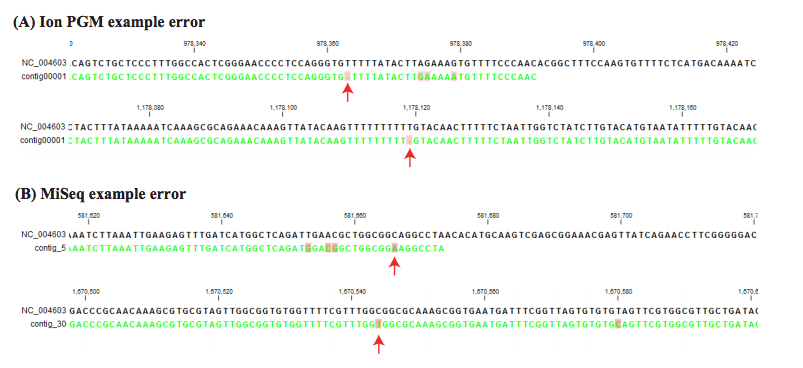
\includegraphics[width=0.8\textwidth]{images/miyamoto_errors}
    \end{center}      
\end{frame}

% Benchmarking results: raw data
\begin{frame}
  \frametitle{Benchmarking on \textit{Vibrio}\footnote{\tiny{Miyamoto \textit{et al}. (2014) \textit{BMC Genomics} \textbf{15}:699 \href{http://dx.doi.org/10.1186/1471-2164-15-699}{doi:10.1186/1471-2164-15-699}}}}
    \begin{center}
      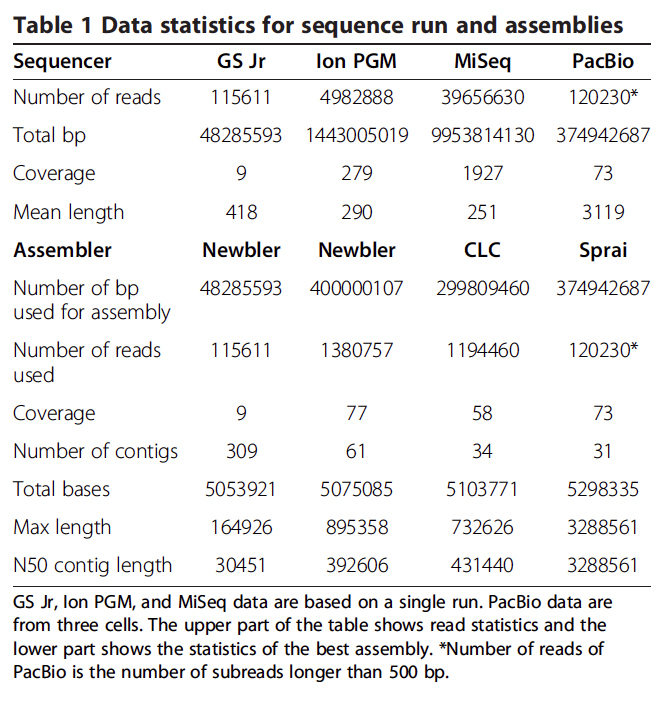
\includegraphics[height=0.8\textheight]{images/miyamoto_table}
    \end{center}      
\end{frame}

% Benchmarking results: alignments
\begin{frame}
  \frametitle{Benchmarking on \textit{Vibrio}\footnote{\tiny{Miyamoto \textit{et al}. (2014) \textit{BMC Genomics} \textbf{15}:699 \href{http://dx.doi.org/10.1186/1471-2164-15-699}{doi:10.1186/1471-2164-15-699}}}}
    \textit{De novo} assembly and alignment against \textit{Vibrio parahaemolyticus} (2x chromosomes)
    \begin{center}
      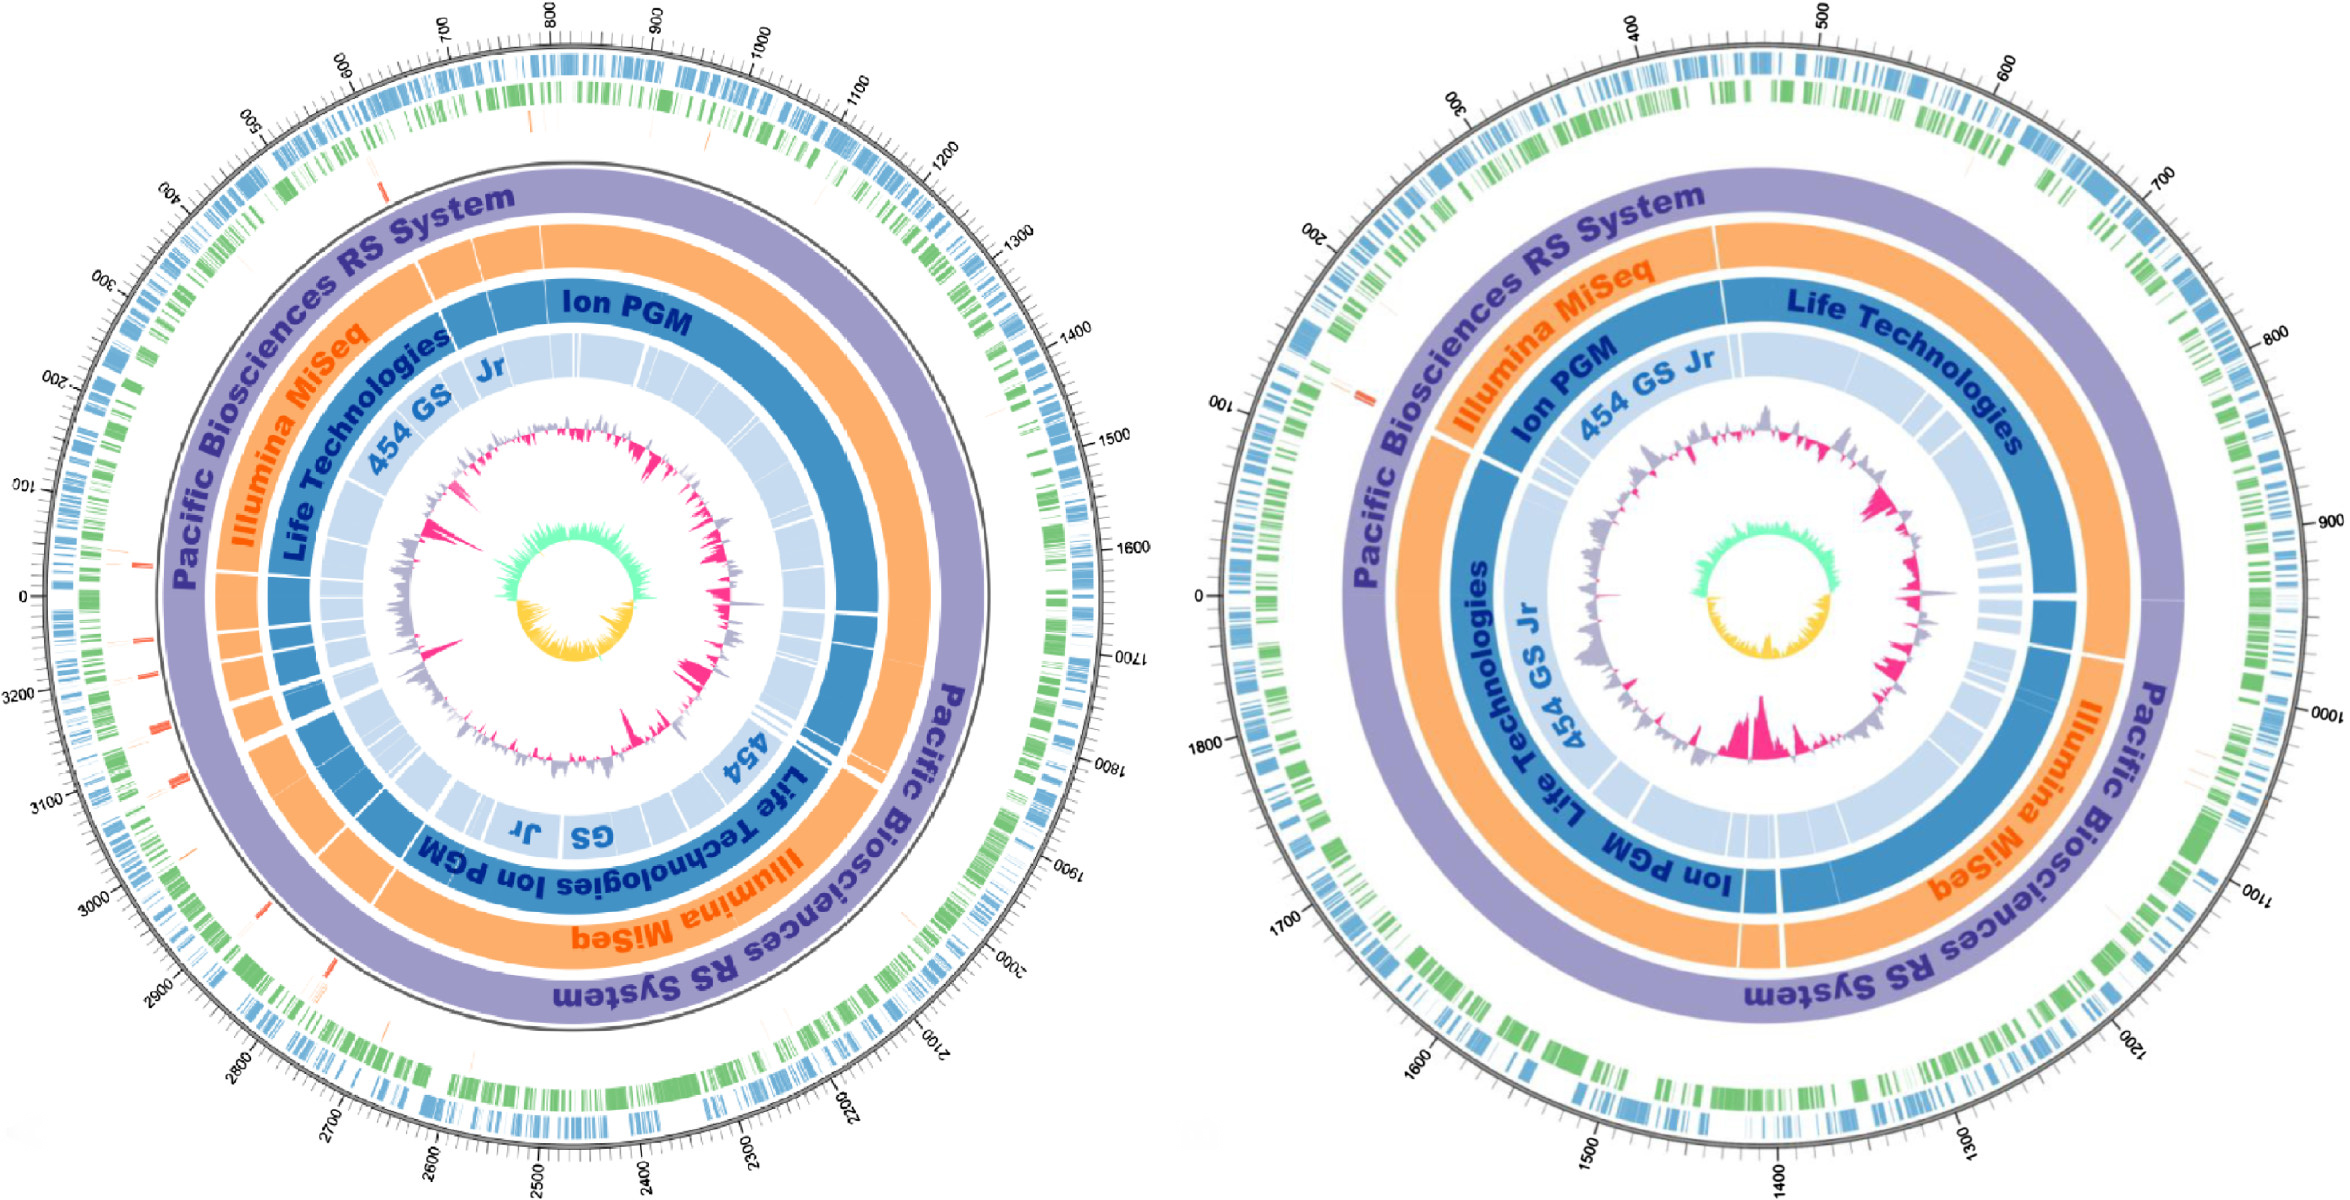
\includegraphics[width=1\textwidth]{images/miyamoto_alignments}
    \end{center}      
\end{frame}

% Benchmarking results: conclusions
\begin{frame}
  \frametitle{Benchmarking on \textit{Vibrio}\footnote{\tiny{Miyamoto \textit{et al}. (2014) \textit{BMC Genomics} \textbf{15}:699 \href{http://dx.doi.org/10.1186/1471-2164-15-699}{doi:10.1186/1471-2164-15-699}}}}
  \begin{itemize}
    \item More and longer reads do not always give the best assemblies: read depth, read distribution also matters
    \item Optimal assemblies were obtained at around 60x-80x coverage (Illumina and Ion).
    \item Multiple rRNA regions are fragmented in short-read assemblies
    \item PacBio generated single chromosome contigs
    \item Assembly of multiple-chromosome bacteria is currently feasible
  \end{itemize}  
  Appreciable variability as methods are not standardised (e.g. sequencing technology, assembler, parameter settings and pre-processing)$\ldots$
\end{frame}

% SUBSECTION: Nanopore
% Brief diversion to Oxford Nanopore
\subsection{Nanopore}

% Nanopore
\begin{frame}
  \frametitle{What's coming next?}
  Oxford Nanopore. A sequencer the size of your hand.
    \begin{center}
      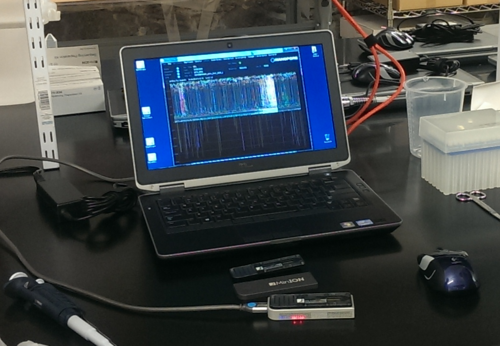
\includegraphics[width=0.48\textwidth]{images/minion_run}\thinspace
      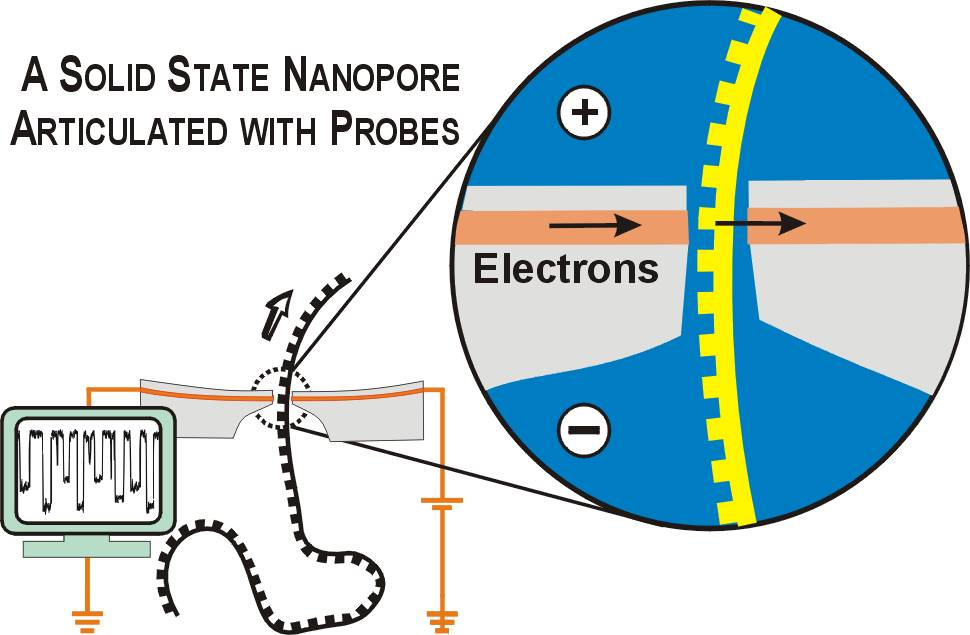
\includegraphics[width=0.48\textwidth]{images/nanopore_schematic}
    \end{center} 
    \begin{itemize}
      \item Microfluidics, single-molecule sequencing; 11-70kbp reads
      \item Reports current across pore (tiny electron microscope) as molecule moves through
      \item \$10/Mbp, 110Mbp per flowcell\footnote{\tiny{Yaniv Erlich (2013) \href{http://erlichya.tumblr.com/post/66376172948/hands-on-experience-with-oxford-nanopore-minion}{Future Continuous blog}}}
    \end{itemize}          
\end{frame}

% Nanopore controversy: paper
\begin{frame}
  \frametitle{Controversy\footnote{\tiny{Mikheyev and Tin (2014) \textit{Mol. Ecol. Res.} \textbf{14}:1097-1102 \href{http://dx.doi.org/10.1111/1755-0998.12324}{doi:10.1111/1755-0998.12324}}}}
  The first Nanopore paper concluded, for $\lambda$ phage:
    \begin{itemize}
      \item About 10\% of reads mapped to the reference genome
      \item \textless1\% of all generated sequence faithfully matches the reference
    \end{itemize}   
    \begin{center}
      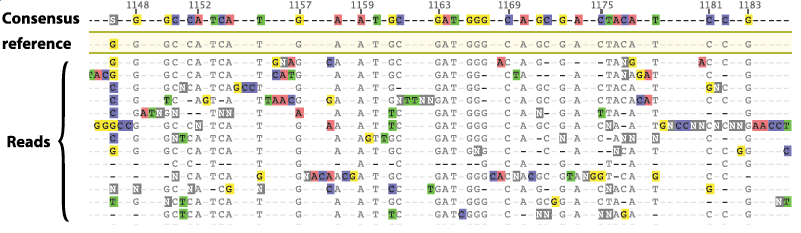
\includegraphics[width=1\textwidth]{images/nanopore_aln}
    \end{center}           
\end{frame}

% Nanopore controversy: response
\begin{frame}
  \frametitle{Controversy\footnote{\tiny{Mikheyev and Tin (2014) \textit{Mol. Ecol. Res.} \textbf{14}:1097-1102 \href{http://dx.doi.org/10.1111/1755-0998.12324}{doi:10.1111/1755-0998.12324}}}}
  Not everyone thinks the Mikheyev and Tin paper is very good:
    \begin{center}
      
\includegraphics[width=0.5\textwidth]{images/nanopore_tweet_1}
      
\includegraphics[width=0.5\textwidth]{images/nanopore_tweet_2}      
    \end{center}           
    \href{http://biomickwatson.wordpress.com/2014/09/07/thoughts-on-oxford-nanopores-minion-mobile-dna-sequencer/}{``But that paper is terrible. It's just lazy.''} (Mick Watson's blog: \href{http://biomickwatson.wordpress.com/2014/09/07/thoughts-on-oxford-nanopores-minion-mobile-dna-sequencer/}{http://biomickwatson.wordpress.com/2014/09/07/thoughts-on-oxford-nanopores-minion-mobile-dna-sequencer/})
\end{frame}

% Some better results
\begin{frame}
  \frametitle{New data\footnote{\tiny{Quick \textit{et al}. (2014) \textit{GigaScience} \textbf{3}:22 \href{http://dx.doi.org/10.1111/1755-0998.12324}{doi:10.1111/1755-0998.12324}}}}
  It's a fast-moving area, and results are improving.
    \begin{center}
      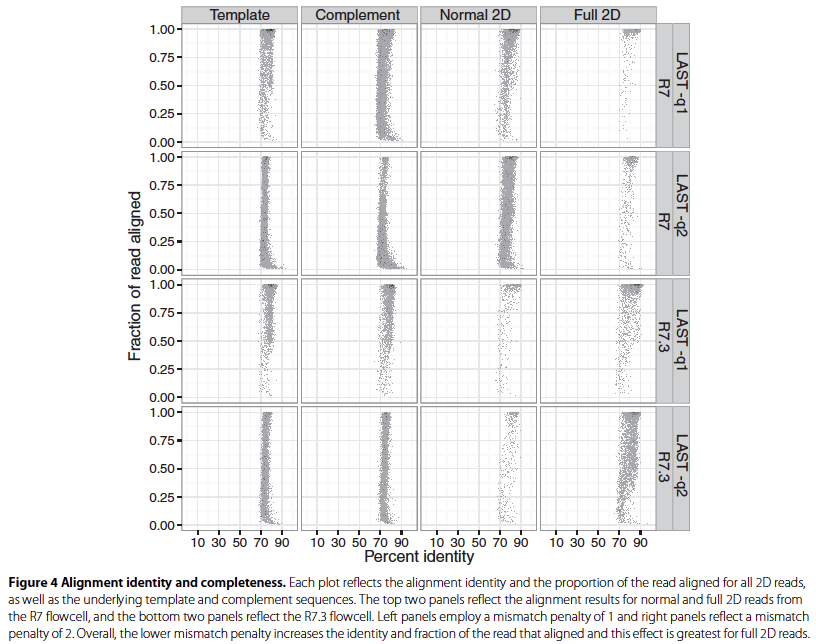
\includegraphics[height=0.65\textheight]{images/nanopore_quick}
    \end{center}           
\end{frame}

% SUBSECTION: How fast is data increasing?
% Summary of how fast the amount of sequence data is increasing
\subsection{How fast is sequence data increasing?}

% How many genomes do we have, now?
\begin{frame}
  \frametitle{After that, the flood$\ldots$}
  High-throughput sequencing methods have completely changed the landscape of microbiology \\
  \textbf{(Nearly) complete, (mainly) accurate sequence data is now inexpensive}
  \begin{itemize}
    \item many more genomes
    \item \href{http://www.genomesonline.org/cgi-bin/GOLD/index.cgi?page_requested=Complete+Genome+Projects&subset_requested=Complete+And+Published}{GOLD} (19/2/2014): 3,011 ``finished'' ; 9,891 ``permanent draft'' genomes
    \item \href{http://www.genomesonline.org/cgi-bin/GOLD/index.cgi?page_requested=Complete+Genome+Projects&subset_requested=Complete+And+Published}{GOLD} (18/11/2014): 6,649 ``finished'' ; 23,552 ``permanent draft'' genomes    
    \item \href{http://www.ncbi.nlm.nih.gov/Traces/wgs/}{NCBI WGS} (19/2/2014): 17,023 microbial genomes
    \item \href{http://www.ncbi.nlm.nih.gov/Traces/wgs/}{NCBI WGS} (18/11/2014): 26,026 micribial genomes
  \end{itemize}
\end{frame}

% And how many are we going to have?
\begin{frame}
  \frametitle{Predicting the future is hard$\ldots$\footnote{\tiny{\href{http://sulab.org/2013/06/sequenced-genomes-per-year/}{http://sulab.org/2013/06/sequenced-genomes-per-year/}}}}
    Su \textit{et al}. attempted to answer this:
    \begin{center}
      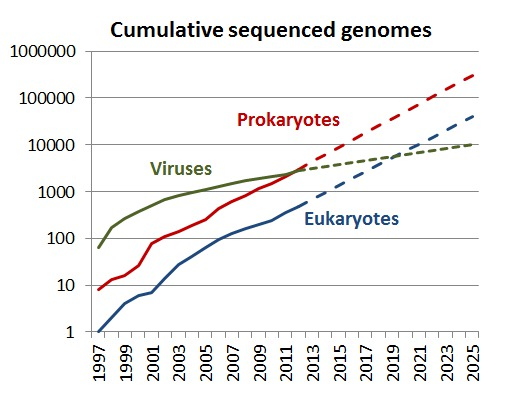
\includegraphics[width=0.5\textwidth]{images/cumulative_sequenced_genomes1}
      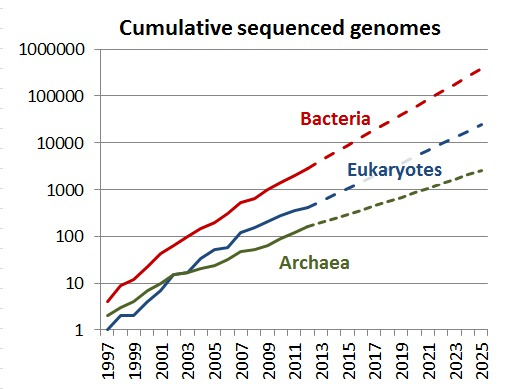
\includegraphics[width=0.5\textwidth]{images/cumulative_sequenced_genomes2}
    \end{center}     
    How will we keep this much genomic data well-organised?
\end{frame}

% SUBSECTION: Genome sequence standard
% Brief account of MIGS
\subsection{Genome Sequence and Data Standards}

% MIGS
\begin{frame}
  \frametitle{MIGS\footnote{\tiny{Field \textit{et al}. (2008) \textit{Nat. Biotech.} \textbf{26}:541-547 \href{http://dx.doi.org/10.1038/nbt.1823}{doi:10.1038/nbt.1823}}}}
  Minimum Information about a (Meta)Genome Sequence (MIGS) \\
  \begin{itemize}
    \item Standardisation of the data describing a genome sequence; standards are \textbf{essential} to data integrity and reuse
    \item Defines core descriptors of the data that cannot be derived from the data (geographical context, experimental methods, etc.)
    \item Produced by \href{http://en.wikipedia.org/wiki/Genomic_Standards_Consortium}{Genomic Standards Consortium} (\href{http://gensc.org/}{gensc.org})
    \item Provided as checklist and XML schema
    \item Now also ``Minimum Information about an ENvironmental Sequence'' (MIENS) and others\footnote{\tiny{Yilmaz \textit{et al}. (2011) \textit{Nat. Biotech.} \textbf{29}:541-547 \href{http://dx.doi.org/10.1038/nbt1360}{doi:10.1038/nbt1360}}}
    \item Global Microbial Identifier (\href{http://www.globalmicrobialidentifier.org/}{http://www.globalmicrobialidentifier.org/})
  \end{itemize}        
\end{frame}

% MIGS table
\begin{frame}
  \frametitle{MIGS\footnote{\tiny{Field \textit{et al}. (2008) \textit{Nat. Biotech.} \textbf{26}:541-547 \href{http://dx.doi.org/10.1038/nbt.1823}{doi:10.1038/nbt.1823}}}}
  Minimum Information about a (Meta)Genome Sequence (MIGS) \\
  \begin{center}
    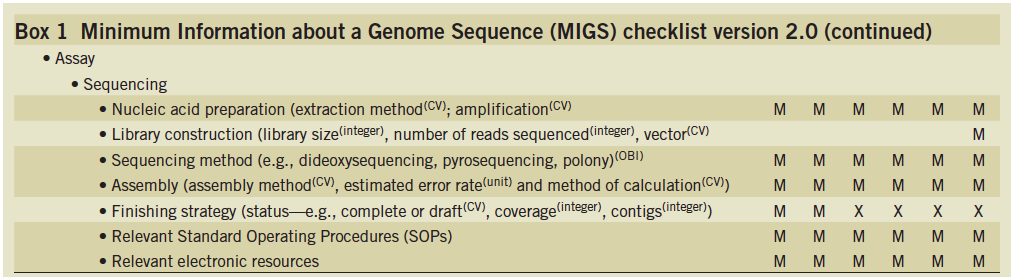
\includegraphics[width=1\textwidth]{images/migs_table}
  \end{center}           
\end{frame}



%%%
% ACKNOWLEDGEMENTS
%\section{Acknowledgements}
%\input{sections/acknowledgements}


%%%
% LICENCE FOR REUSE
%% licence.tex
%% Author: Leighton Pritchard
%% Copyright: James Hutton Institute
%% These slides describe the licence for reuse of these slides and
%% materials

%
\begin{frame}
  \frametitle{Licence: CC-BY-SA}
  By: Leighton Pritchard \\[0.5cm]
  This presentation is licensed under the Creative Commons Attribution ShareAlike license \\
  \href{https://creativecommons.org/licenses/by-sa/4.0/}{https://creativecommons.org/licenses/by-sa/4.0/}
\end{frame}

% etc
\end{document}